%%%%%%%%%%%%%%%%%%%%%%%%%%%%%%%%%%%%%%%%%%%%%%%%%%%%%%%%%%%%%%%%%%%%%
%
% Complete documentation on the extended LaTeX markup used for Insight
% documentation is available in ``Documenting Insight'', that is part
% of the standard documentation for Insight.  It may be found online
% at:
%
%                    http://www.itk.org
%
%%%%%%%%%%%%%%%%%%%%%%%%%%%%%%%%%%%%%%%%%%%%%%%%%%%%%%%%%%%%%%%%%%%%%

\documentclass{InsightSoftwareGuide}

\usepackage[dvips]{graphicx}
\usepackage{times}
\usepackage{color}
\usepackage{listings}
\usepackage{minted}
\usepackage{setspace}
\usepackage{hyphenat}
\usepackage[toc,page]{appendix}
\usepackage{verbatim}
\usepackage{imakeidx}

\usepackage{draftwatermark}
%\usepackage[firstpage]{draftwatermark}
\SetWatermarkText{DRAFT-ITK}%default is DRAFT
\SetWatermarkLightness{0.90}%default is 0.8
\SetWatermarkScale{0.8}%default is 1.2

%\allowhyphens

\lstnewenvironment{itklisting}
{\singlespacing\lstset{language=C++}}
{}

\definecolor{ltgray}{rgb}{0.97,0.97,0.97}
\usemintedstyle{emacs}

\lstset{
         basicstyle=\footnotesize\ttfamily, % Standardschrift
         %numbers=left,               % Ort der Zeilennummern
         numberstyle=\tiny,          % Stil der Zeilennummern
         %stepnumber=2,               % Abstand zwischen den Zeilennummern
         numbersep=2pt,              % Abstand der Nummern zum Text
         tabsize=2,                  % Groesse von Tabs
         extendedchars=true,         %
         breaklines=true,            % Zeilen werden Umgebrochen
         keywordstyle=\color{red},
 %    frame=b,
 %        keywordstyle=[1]\textbf,    % Stil der Keywords
 %        keywordstyle=[2]\textbf,    %
 %        keywordstyle=[3]\textbf,    %
 %        keywordstyle=[4]\textbf,   \sqrt{\sqrt{}} %
         stringstyle=\color{black}\ttfamily, % Farbe der String
         showspaces=false,           % Leerzeichen anzeigen ?
         showtabs=false,             % Tabs anzeigen ?
         xleftmargin=17pt,
         framexleftmargin=17pt,
         framexrightmargin=5pt,
         framexbottommargin=4pt,
         backgroundcolor=\color{ltgray},
         showstringspaces=false      % Leerzeichen in Strings anzeigen ?
 }

 \lstloadlanguages{% Check Dokumentation for further languages ...
         %[Visual]Basic
         %Pascal
         %C
         C++
         %XML
         %HTML
         %Java
 }
%\DeclareCaptionFont{blue}{\color{blue}}

%\captionsetup[lstlisting]{singlelinecheck=false, labelfont={blue}, textfont={blue}}
\usepackage{caption}
\DeclareCaptionFont{white}{\color{white}}
\DeclareCaptionFormat{listing}{\colorbox[cmyk]{0.43, 0.35, 0.35,0.01}{\parbox{\textwidth}{\hspace{15pt}#1#2#3}}}
\captionsetup[lstlisting]{format=listing,labelfont=white,textfont=white, singlelinecheck=false, margin=0pt, font={bf,footnotesize}}

\newif\ifitkFullVersion
\itkFullVersiontrue
%\itkFullVersionfalse


%%%%%%%%%%%%%%%%%%%%%%%%%%%%%%%%%%%%%%%%%%%%%%%%%%%%%%%%%%%%%%%%%%%
%
%
%   Load configuration parameters prepared by CMake
%
%
%%%%%%%%%%%%%%%%%%%%%%%%%%%%%%%%%%%%%%%%%%%%%%%%%%%%%%%%%%%%%%%%%%%

\input{SoftwareGuideConfiguration.tex}

%%%%%%%%%%%%%%%%%%%%%%%%%%%%%%%%%%%%%%%%%%%%%%%%%%%%%%%%%%%%%%%%%%
%
%  hyperref should be the last package to be loaded.
%
%%%%%%%%%%%%%%%%%%%%%%%%%%%%%%%%%%%%%%%%%%%%%%%%%%%%%%%%%%%%%%%%%%
\ifitkPrintedVersion
\usepackage[dvips,
pdftitle={ITK Software Guide},
pdfauthor={Hans Johnson and Luis Ib'{a}~{n}ez and Matthew McCormick and the Insight Software Consortium},
pdfsubject={Medical Image Segmentation and Registration Toolkit}
pdfkeywords={Registration,Segmentation,Guide},
pdfpagemode={UseOutlines},
bookmarks,bookmarksopen,
pdfstartview={FitH},
backref,
colorlinks,linkcolor={black},citecolor={black},urlcolor={black},
]{hyperref}
\else
\usepackage[dvips,
pdftitle={ITK Software Guide},
pdfauthor={Hans Johnson and Luis Ib'{a}~{n}ez and Matthew McCormick and the Insight Software Consortium},
pdfsubject={Medical Image Segmentation and Registration Toolkit},
pdfkeywords={Registration,Segmentation,Guide},
pdfpagemode={UseOutlines},
bookmarks,bookmarksopen,
pdfstartview={FitH},
backref,
colorlinks,linkcolor={blue},citecolor={blue},urlcolor={blue},
]{hyperref}
\fi

%%%%%%%%%%%%%%%%%%%%%%%%%%%%%%%%%%%%%%%%%%%%%%%%%%%%%%%%%%%%%%%%%%%
%
%
%           The Insight Toolkit Software Guide
%
%
%%%%%%%%%%%%%%%%%%%%%%%%%%%%%%%%%%%%%%%%%%%%%%%%%%%%%%%%%%%%%%%%%%%

\author{Hans J. Johnson, Matthew M. McCormick, Luis Ib\'{a}\~{n}ez, and the \emph{Insight Software Consortium}}

\authoraddress{
  \url{http://itk.org}\\
  Email: \email{community@itk.org}
}

\date{\today}

% actually write the .idx file
\makeindex

\setcounter{tocdepth}{3}



\title{The ITK Software Guide\\Book 2: Design and Functionality\\Fourth Edition\\ \emph{Updated for ITK version
\ITKVERSIONMAJORMINOR}}


%%%%%%%%%%%%%%%%%%%%%%%%%%%%%%%%%%%%%%%%%%%%%%%%%%%%%%%%%%%%%%%%%%%
%
%           Begin Document
%
%%%%%%%%%%%%%%%%%%%%%%%%%%%%%%%%%%%%%%%%%%%%%%%%%%%%%%%%%%%%%%%%%%%

\begin{document}

\ifitkPrintedVersion

  \begin{minipage}[t][3cm][b]{\textwidth}
  \rule{14cm}{1pt}
  \end{minipage}

  \begin{minipage}[t][3cm][b]{\textwidth}
  \Huge
  The ITK Software Guide\\
  Book 2: Design and Functionality\\
  \normalsize
  \par
  \emph{Updated for version \ITKVERSIONMAJORMINOR}\\

  \end{minipage}

  \hfill
\begin{minipage}[t][6cm][b]{0.6\textwidth}
\Large
\renewcommand{\baselinestretch}{1.5}
Hans J. Johnson\\
Matthew McCormick \\
Luis Ib\'{a}\~{n}ez\\
and the \emph{Insight Software Consortium}
\normalsize
\end{minipage}


\begin{minipage}[t][2cm][b]{\textwidth}
\rule{14cm}{1pt}
\end{minipage}

\newpage

\begin{minipage}[t][4cm][b]{\textwidth}
\begin{center}
\includegraphics[width=0.5\textwidth]{Kitware-logo-medium-res.eps}
\end{center}
\par
\begin{center}
\large

\copyright \the\year \; Kitware, Inc. \emph{(cover, preface, postface)}\\
\copyright \the\year \; Insight Software Consortium \emph{(main text body)}\\
Published by Kitware, Inc. \texttt{http://www.kitware.com}
\normalsize
\end{center}
\end{minipage}


\begin{minipage}[t][2.25cm][b]{\textwidth}
\begin{center}
An electronic version of this document is available from
\texttt{https://itk.org}.
\end{center}
\begin{tabular}{p{.9\textwidth}}
This work is licensed under a Creative Commons Attribution 3.0 Unported License.
\begin{center}
\includegraphics[width=3.4cm]{cc-by.eps}
\end{center}\\
\end{tabular}
\end{minipage}


\begin{minipage}[t][2.5cm][b]{\textwidth}
\begin{center}
This project has been funded in whole or in part with Federal funds from the
National Institutes of Health (NLM, NIDCR, NIMH, NEI, NINDS, NIDCD, NCI), the
NSF, and the DoD (TATRC). Funding has primarily come under the direction of the
National Library of Medicine, National Institutes of Health, under numerous
contracts. Recently, the major revision to the toolkit, ITKv4, was made
possible by NLM directed funds from the American Reinvestment and Recovery Act
(ARRA).
\end{center}
\end{minipage}


\begin{minipage}[t][1.0cm][b]{\textwidth}
\begin{center}
All product names mentioned herein are the trademarks of their respective
owners.
\end{center}
\end{minipage}


\begin{minipage}[t][2.7cm][b]{\textwidth}
\begin{center}
Document created with \LaTeX{}, using CMake as
configuration manager, with a Python script to extract examples from the
\code{ITK/Examples} directory. All code in this document compiled at
the time of publication.
\end{center}
\end{minipage}

  \begin{minipage}[t][1.0cm][b]{\textwidth}
\begin{center}
Printed and produced in the United States of America.\\
\textbf{ISBN 978-1-930934-36-8}
\end{center}
\end{minipage}


\fi

\maketitle

\frontmatter

\hyperbaseurl{http://www.itk.org/Insight}


%%%%%%%%%%%%%%%%%%%%%%%%%%%%%%%%%%%%%%%%%%
%
%  Page with Quote and ITK Logo
%
%
%%%%%%%%%%%%%%%%%%%%%%%%%%%%%%%%%%%%%%%%%%
\cleardoublepage

\begin{minipage}[t][10cm][b]{\textwidth}
\center
\includegraphics[width=0.5\textwidth]{itkLogo.eps}
\large
\begin{center}
\emph{The purpose of computing is Insight, not numbers.}\\
\end{center}
\hspace{8cm} Richard Hamming
\normalsize
\end{minipage}



%%%%%%%%%%%%%%%%%%%%%%%%%%%%%%%%%%%%%%%%%%%%%%
%
% remove headings from the following material
\pagestyle{plain}
%
%%%%%%%%%%%%%%%%%%%%%%%%%%%%%%%%%%%%%%%%%%%%%%


\ifitkPrintedVersion
  % We want this material to fit on two pages
\small

\chapter*{About the Cover}

The cover image consists of a photograph of ABS plastic anatomical objects
printed with a MakerBot Replicator 2X 3D printer. Mesh STL files were generated from the images with VTK.

\begin{description}

\item [Skull.]
Given that the origins of ITK are with the Visible Human Project, it is
appropriate that the skull was derived from the Visible Woman dataset. The
skull was segmented with ITK from the Visible Woman head CT images with simple
thresholding\footnote{\url{https://github.com/XiaoxiaoLiu/3D-printing}}.

\item[Brain.]
The brain model was segmented with ITK as described in the open science
publication:
\begin{quote}
McCormick M, Liu X, Jomier J, Marion C and Ibanez L. ITK:
enabling reproducible research and open science. Front. Neuroinform. 8:13.
2014. doi: 10.3389/fninf.2014.00013
\end{quote}

\end{description}

\normalsize

\fi

\ifitkFullVersion
  \chapter*{Abstract}
\noindent
The Insight Toolkit \href{http://itk.org}{(ITK)} is an open-source
software toolkit for performing registration and
segmentation. \emph{Segmentation} is the process of identifying and
classifying data found in a digitally sampled
representation. Typically the sampled representation is an image
acquired from such medical instrumentation as CT or MRI
scanners. \emph{Registration} is the task of aligning or developing
correspondences between data. For example, in the medical environment,
a CT scan may be aligned with a MRI scan in order to combine the
information contained in both.

ITK is a cross-platform software. It uses a build environment known as
\href{http://cmake.org}{CMake} to manage platform-specific project
generation and compilation process in a platform-independent way. ITK is
implemented in C++. ITK's implementation style employs generic programming,
which involves the use of templates to generate, at compile-time, code that can
be applied \emph{generically} to any class or data-type that supports the
operations used by the template. The use of C++ templating means that the code
is highly efficient and many issues are discovered at compile-time, rather than
at run-time during program execution. It also means that many of ITK's
algorithms can be applied to arbitrary spatial dimensions and pixel types.

An automated wrapping system integrated with ITK generates an interface between
C++ and a high-level programming language \href{http://www.python.org}{Python}.
This enables rapid prototyping and faster exploration of ideas by shortening the
edit-compile-execute cycle. In addition to automated
wrapping, the \href{http://www.itk.org/Wiki/SimpleITK}{SimpleITK} project
provides a streamlined interface to ITK that is available for C++, Python, Java,
CSharp, R, Tcl and Ruby.

Developers from around the world can use, debug, maintain, and extend the
software because ITK is an open-source project. ITK uses a
model of software development known as Extreme
Programming. Extreme Programming collapses the usual software development
methodology into a simultaneous iterative process of
design-implement-test-release. The key features of Extreme Programming
are communication and testing. Communication among the members of the
ITK community is what helps manage the rapid evolution of the
software. Testing is what keeps the software stable. An
extensive testing process supported by the system known as
\href{http://open.cdash.org/index.php?project=Insight}{CDash}
measures the quality of ITK code on a daily basis. The ITK Testing Dashboard is
updated continuously, reflecting the quality of the code at any moment.

The most recent version of this document is available online at
\url{http://itk.org/ItkSoftwareGuide.pdf}.

  This book is a guide to developing software with ITK; it is the second of two
companion books. This book covers detailed design and functionality for
reading and writing images, filtering, registration, segmentation, and
performing statistical analysis. The first book covers building and installation, general
architecture and design, as well as the process of contributing in the ITK
community.

  \chapter*{Contributors}
\noindent

The Insight Toolkit \href{http://www.itk.org}{(ITK)} has been created by the
efforts of many talented individuals and prestigious organizations. It is also
due in great part to the vision of the program established by Dr. Terry Yoo
and Dr. Michael Ackerman at the National Library of Medicine.

This book lists a few of these contributors in the following paragraphs. Not
all developers of ITK are credited here, so please visit the Web pages at
\href{http://www.itk.org/HTML/About.htm}{http://www.itk.org/HTML/About.htm}
for the names of additional contributors, as well as checking the GIT source
logs for code contributions.

The following is a brief description of the contributors to this software
guide and their contributions.


{\bf Luis Ib\'{a}\~{n}ez} is principal author of this text.
He assisted in the design and layout of the text, implemented the bulk of
the \LaTeX{} and CMake build process, and was responsible for the bulk of
the content. He also developed most of the example code found in the
\code{Insight/Examples} directory.

{\bf Will Schroeder} helped design and establish the organization
of this text and the \code{Insight/Examples} directory. He is principal
content editor, and has authored several chapters.

{\bf Lydia Ng} authored the description for the registration framework
and its components, the section on the multiresolution framework, and
the section on deformable registration methods. She also edited the
section on the resampling image filter and the sections on various
level set segmentation algorithms.

{\bf Joshua Cates} authored the iterators chapter and the text and examples
describing watershed segmentation. He also co-authored the level-set
segmentation material.

{\bf Jisung Kim} authored the chapter on the statistics framework.

{\bf Julien Jomier} contributed the chapter on spatial objects and examples on
model-based registration using spatial objects.

{\bf Karthik Krishnan} reconfigured the process for automatically generating
images from all the examples. Added a large number of new examples and updated
the Filtering and Segmentation chapters for the second edition.

{\bf Stephen Aylward} contributed material describing spatial objects and
their application.

{\bf Tessa Sundaram} contributed the section on deformable registration using
the finite element method.

{\bf YinPeng Jin} contributed the examples on  hybrid segmentation methods.

{\bf Celina Imielinska} authored the section describing the principles of
hybrid segmentation methods.

{\bf Mark Foskey} contributed the examples on the
AutomaticTopologyMeshSource class.

{\bf Mathieu Malaterre} contributed the entire section on the description and
use of DICOM readers and writers based on the GDCM library. He also contributed
an example on the use of the VTKImageIO class.

{\bf Gavin Baker} contributed the section on how to write composite filters.
Also known as minipipeline filters.

Since the software guide is generated in part from the ITK source code
itself, many ITK developers have been involved in updating and
extending the ITK documentation.  These include {\bf David Doria},
{\bf Bradley Lowekamp}, {\bf Mark Foskey}, {\bf Ga\"{e}tan Lehmann},
{\bf Andreas Schuh}, {\bf Tom Vercauteren}, {\bf Cory Quammen}, {\bf Daniel Blezek},
{\bf Paul Hughett}, {\bf Matthew McCormick}, {\bf Josh Cates}, {\bf Arnaud Gelas},
{\bf Jim Miller}, {\bf Brad King}, {\bf Gabe Hart}, {\bf Hans Johnson}.

{\bf Hans Johnson}, {\bf Kent Williams}, {\bf Constantine Zakkaroff}, {\bf
Xiaoxiao Liu}, {\bf Ali Ghayoor}, and {\bf Matthew McCormick} updated
the documentation for the initial ITK version 4 release.

\fi



%%%%%%%%%%%%%%%%%%%%%%%%%%%%%%%%%%%%%%%%%%%%%%%%%%%%%%%%%
%
% Insert Table of Contents; List of Figures and Tables
%
%%%%%%%%%%%%%%%%%%%%%%%%%%%%%%%%%%%%%%%%%%%%%%%%%%%%%%%%%


%%%%%%%%%%%%%%%%%%%%%%%%%%%%%%%%%%%%%%%%%%%%%%
%
% enable headings from the following material
\pagestyle{normal}
%
%%%%%%%%%%%%%%%%%%%%%%%%%%%%%%%%%%%%%%%%%%%%%%
\small
\tableofcontents
\listoffigures
\listoftables
\normalsize


%%%%%%%%%%%%%%%%%%%%%%%%%%%%%%%%%%%%%%%%%
%
% Begin technical content
%
%%%%%%%%%%%%%%%%%%%%%%%%%%%%%%%%%%%%%%%%%

\mainmatter

\input{DF01-IO.tex}
\input{DF02-Filtering.tex}
\chapter{Registration}

\begin{floatingfigure}[rlp]{8cm}
  \centering
  \includegraphics[width=8cm]{ImageRegistrationConcept.eps}
  \caption[Image Registration Concept]{Image registration is the task of
finding a spatial transform mapping on image into
another.\label{fig:ImageRegistrationConcept}}
\end{floatingfigure}

This chapter introduces ITK's capabilities for performing image
registration. Image registration is the process of determining the spatial
transform that maps points from one image to homologous points on a object in
the second image. This concept is schematically represented in Figure
\ref{fig:ImageRegistrationConcept}. In ITK, registration is performed within
a framework of pluggable components that can easily be interchanged.  This
flexibility means that a combinatorial variety of registration methods can be
created, allowing users to pick and choose the right tools for their specific
application.


\section{Registration Framework}
Let's begin with a simplified typical registration framework where its components
and their interconnections are shown in Figure \ref{fig:RegistrationComponents}.
The basic input data to the registration process are two images: one is defined
as the \emph{fixed} image $f(\bf{X})$ and the other as the \emph{moving} image
$m(\bf{X})$, where $\bf{X}$ represents a position in N-dimensional space.
Registration is treated as an optimization problem with the goal of finding the
spatial mapping that will bring the moving image into alignment with the fixed image.

\begin{figure}
\center
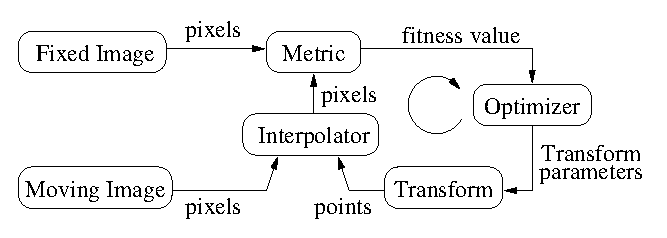
\includegraphics[width=0.8\textwidth]{RegistrationComponentsDiagram.eps}
\itkcaption[A Typical Registration Framework Components]{The basic components
of a typical registration framework are two input images, a transform, a
metric, an interpolator and an optimizer.}
\label{fig:RegistrationComponents}
\end{figure}

The \emph{transform} component $T(\bf{X})$ represents the spatial mapping of
points from the fixed image space to points in the moving image space. The
\emph{interpolator} is used to evaluate moving image intensities at non-grid
positions. The \emph{metric} component $S(f,m \circ T)$ provides a measure of
how well the fixed image is matched by the transformed moving image. This
measure forms the quantitative criterion to be optimized by the
\emph{optimizer} over the search space defined by the parameters of the
\emph{transform}.

The ITKv4 registration framework provides more flexibility to the above traditional
registration concept. In this new framework, specifications of the registration
matching metric comparison locations can be completely different from the pixel
sampling locations in the fixed image.
This means that the registration computations can happen on a physical grid
completely different than the fixed image domain and sampling desity.
This sampling domain can be considered as a new component in the registration
framework known as a \textbf{virtual image}. Moreover, the matching metric
does not need to be computed on a uniform grid of points; it can be computed
on an arbitrary set of physical points.

Various ITKv4 registration components are illustrated in Figure
\ref{fig:ITKv4RegistrationComponents}. Boxes with dashed borders show
\emph{data objects}, while those with solid borders show \emph{process objects}.

\begin{figure}
\center
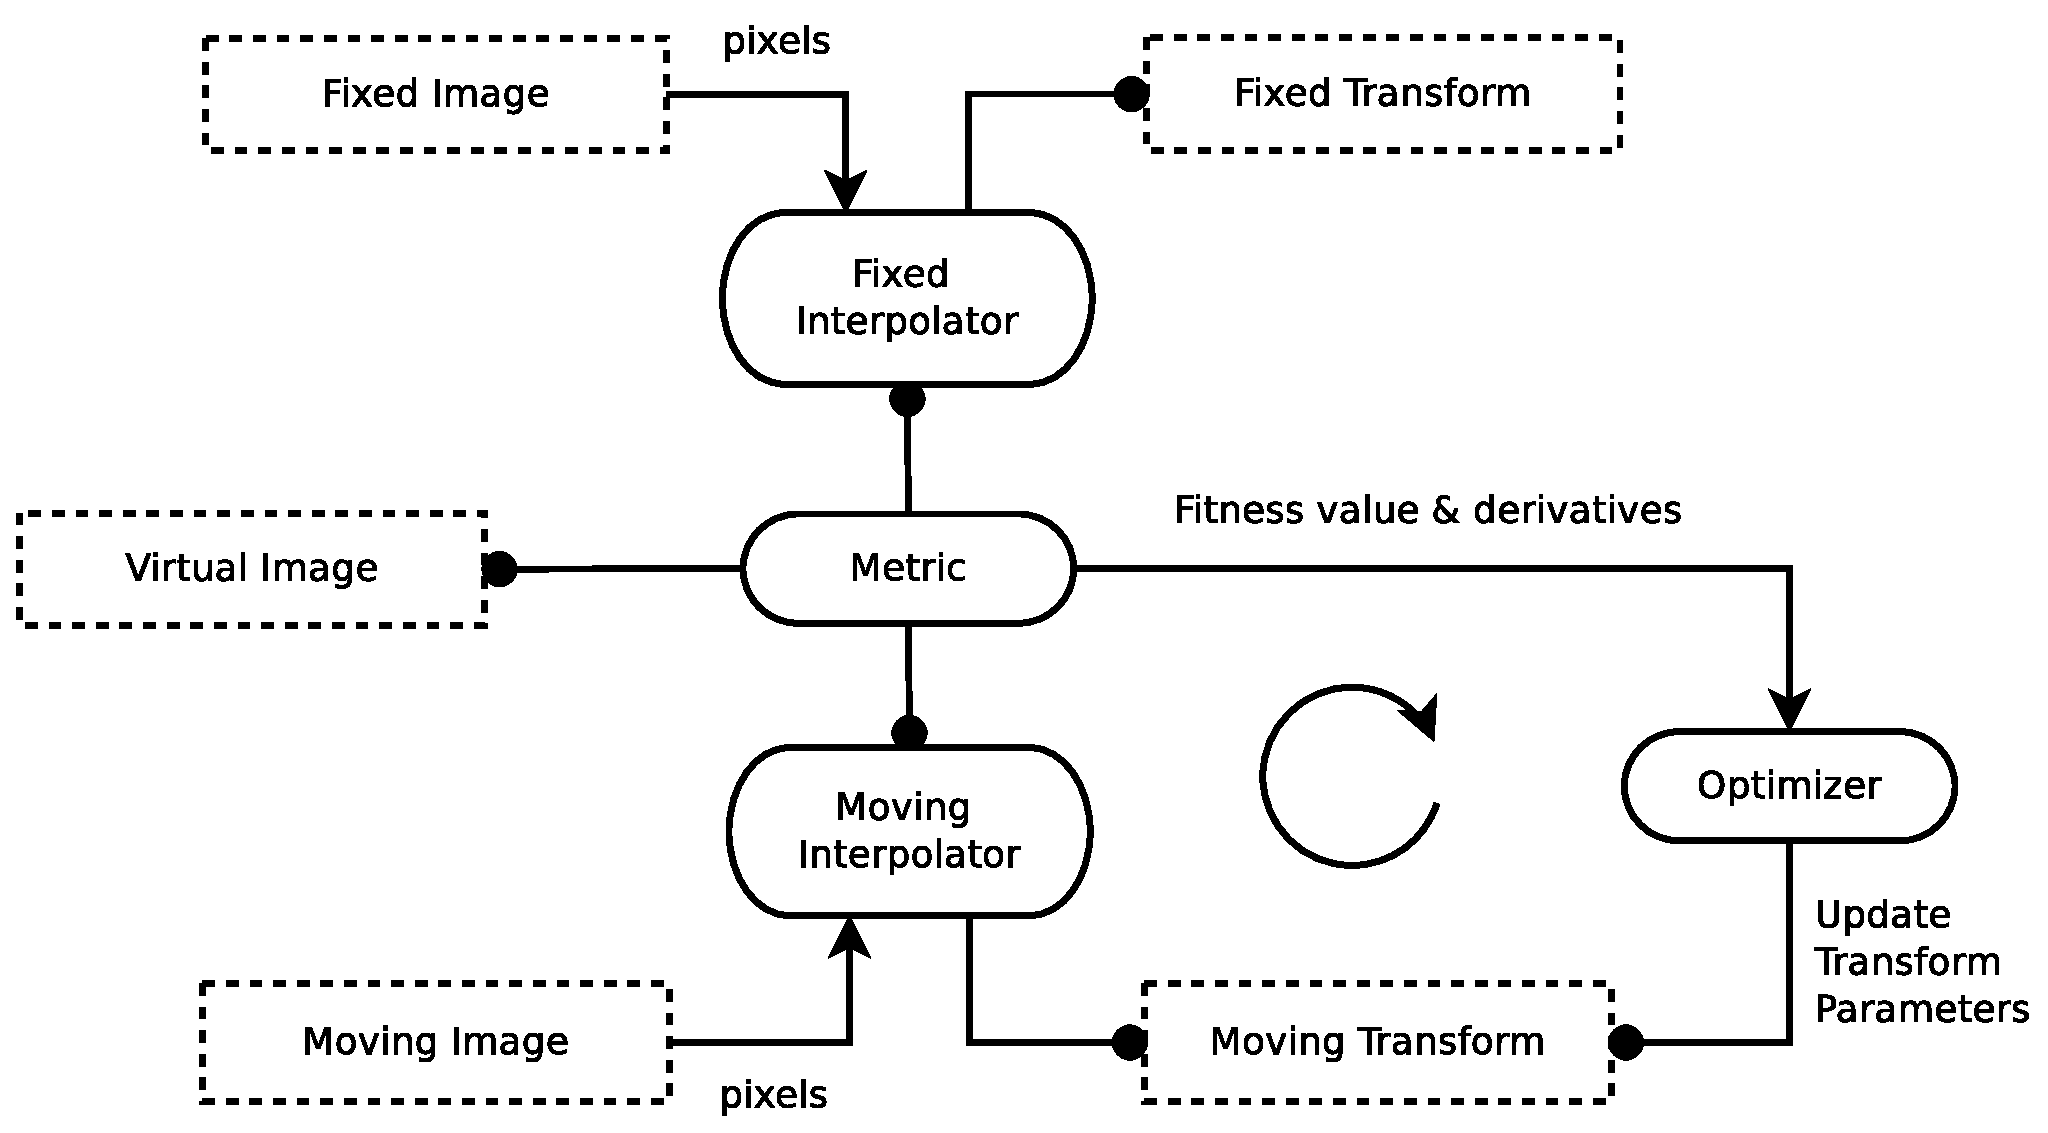
\includegraphics[width=0.8\textwidth]{ITKv4RegistrationComponentsDiagram.eps}
\itkcaption[Registration Framework Components]{The basic components of the ITKv4
registration framework.}
\label{fig:ITKv4RegistrationComponents}
\end{figure}

The matching Metric class is a key component that controls most parts of the
registration process since it handles fixed, moving and virtual images as well
as fixed and moving transforms and interpolators.

Fixed and moving transforms and interpolators are used by the metric to evaluate
the intensity values of the fixed and moving images at each physical point of the
virtual space. Those intensity values are then used by the metric cost function to
evaluate its fitness value and derivatives, which are passed to the optimizer that
asks the moving transform to update its parameters based on the outputs of the cost
function. Since the moving transform is shared between metric and optimizer,
the above process will be repeated till the convergence criteria are met.

Later in section~\ref{sec:FeaturesOfTheRegistrationFramework} you will get a
better understanding of the behind-the-scenes processes of ITKv4 registration
framework. First, we begin with some simple registration examples.


\section{"Hello World" Registration}
\label{sec:IntroductionImageRegistration}
\ifitkFullVersion
\input{ImageRegistration1.tex}
\fi

\section{Features of the Registration Framework}
\label{sec:FeaturesOfTheRegistrationFramework}

This section presents internals of the registration process in ITKv4.
Understanding what actually happens is necessary to have a correct interpretation
of the results of a registration filter. It also helps to understand the
most common difficulties that users encounter when they start using the ITKv4
registration framework:

\begin{itemize}
\item Registration is done in physical coordinates
\item The direction of the transform maps from the space of the virtual image to that of the moving image
\end{itemize}

These two topics tend to create confusion because they
are implemented in different ways in other systems, and community members tend to
have different expectations regarding how registration should work in ITKv4. The
situation is further complicated by the way most people describe image
operations, as if they were manually performed on a continuous picture on a piece
of paper.

These concepts are discussed in this section through a general example shown in
Figure~\ref{fig:ImageRegistrationCoordinateSystemsDiagram}.

\begin{figure}
\center
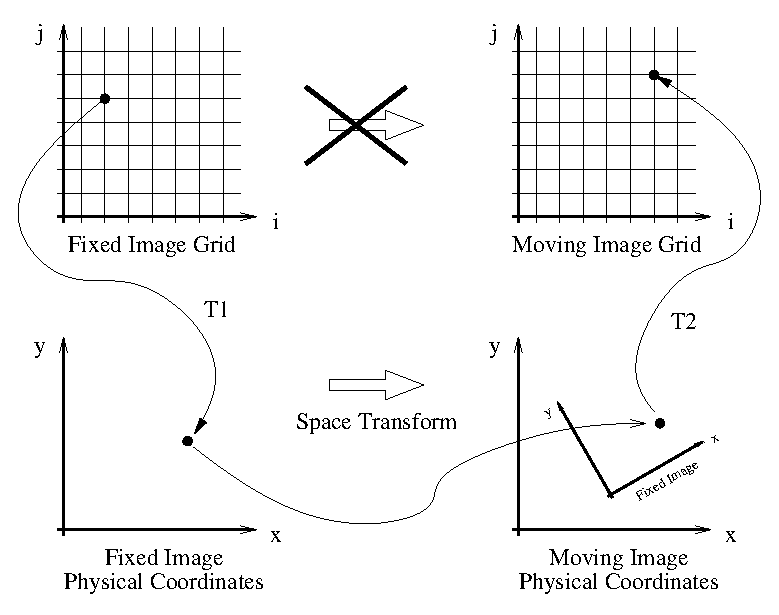
\includegraphics[width=0.75\textwidth]{ImageRegistrationCoordinateSystemsDiagram.eps}
\itkcaption[Registration Coordinate Systems]{Different coordinate systems
involved in the image registration process. Note that the transform being
optimized is the one mapping from the physical space of the \textbf{virtual}
image into the physical space of the \textbf{moving} image.}
\label{fig:ImageRegistrationCoordinateSystemsDiagram}
\end{figure}

Recall that ITKv4 does the registration in ``physical'' space where fixed,
moving and virtual images are placed. Also, note that the term of
virtual image is deceptive here since it does not refer to any actual
image. In fact, the virtual image defines the origin, direction and the
spacing of a space lattice that holds the output resampled image of the
registration process. The virtual pixel lattice is illustrated in green
at the top left side of
Figure~\ref{fig:ImageRegistrationCoordinateSystemsDiagram}.

As shown in this figure, generally there are two transforms involved in the
registration process even though only one of them is being optimized. $T_{vm}$
maps points from physical virtual space onto the physical space of the moving
image, and in the same way $T_{vf}$ finds homologous points between physical
virtual space and the physical space of the fixed image. Note that only
$T_{vm}$ is optimized during the registration process. $T_{vf}$ cannot be
optimized. The fixed transform usually is an identity transform since the
virtual image lattice is commonly defined as the fixed image lattice.

When the registration starts, the algorithm goes through each grid point of the
virtual lattice in a raster sweep. At each point the fixed
and moving transforms find coordinates of the homologous points in the fixed
and moving image physical spaces, and interpolators are used to find the pixel
intensities if mapped points are in non-grid positions. These intensity values
are passed to a cost function to find the current metric value.

Note the direction of the mapping transforms here. For example,
if you consider the $T_{vm}$ transform, confusion often occurs since
the transform shifts a virtual lattice point on the \textbf{positive}
X direction. The visual effect of this mapping, once the moving
image is resampled, is equivalent to manually shifting the moving
image along the \textbf{negative} X direction. In the same way, when
the $T_{vm}$ transform applies a \textbf{clock-wise} rotation to the
virtual space points, the visual effect of this mapping, once the
moving image has been resampled, is equivalent to manually rotating
the moving image \textbf{counter-clock-wise}. The same relationships
also occur with the $T_{vf}$ transform between the virtual space and
the fixed image space.

This mapping direction is chosen because the moving image is resampled
on the grid of the virtual image. In the resampling process,
an algorithm iterates through every pixel of the output image
and computes the intensity assigned to this pixel by
mapping to its location in the moving image.

Instead, if we were to use the transform mapping coordinates from the
moving image physical space into the virtual image physical space,
then the resampling process would not guarantee that every pixel in
the grid of the virtual image would receive one and only one value.
In other words, the resampling would result in an image with
holes and redundant or overlapping pixel values.

As seen in the previous examples, and as corroborated in the remaining
examples in this chapter, the transform computed by the registration
framework can be used directly in the resampling filter in order to
map the moving image onto the discrete grid of the virtual image.

There are exceptional cases in which the transform desired is actually
the inverse transform of the one computed by the ITK registration framework.
Only those cases may require invoking the \code{GetInverse()}
method that most transforms offer. Before attempting this,
read the examples on resampling illustrated in
section~\ref{sec:GeometricalTransformationFilters} in order to
familiarize yourself with the correct interpretation of the transforms.

Now we come back to the situation illustrated in
Figure~\ref{fig:ImageRegistrationCoordinateSystemsDiagram}. This figure shows
the flexibility of the ITKv4 registration framework. We can register two
images with different scales, sizes and resolutions. Also, we can create the
output warped image with any desired size and resolution.

Nevertheless, note that the spatial transform computed during the
registration process does not need to be concerned about a different number
of pixels and different pixel sizes between fixed, moving and output images
because the conversion from index space to the physical space implicitly
takes care of the required scaling factor between the involved images.

One important consequence of this fact is that having the correct image origin,
image pixel size, and image direction is fundamental for the success of the
registration process in ITK, since we need this information to compute the exact
location of each pixel lattice in the physical space; we must make sure
that the correct values for the origin, spacing, and direction of all
fixed, moving and virtual images are provided.

In this example, the spatial transform computed will \textbf{physically} map
the brain from the moving image onto the virtual space and minimize its
difference with the resampled brain from the fixed image into the virtual
space. Fortunately in practice there is no need to resample the fixed image
since the virtual image physical domain is often assumed to be the same as
physical domain of the fixed image.

\section{Monitoring Registration}
\label{sec:MonitoringImageRegistration}
\ifitkFullVersion
\input{ImageRegistration3.tex}
\fi



\section{Multi-Modality Registration}
\label{sec:MultiModalityRegistration}

Some of the most challenging cases of image registration arise when images of
different modalities are involved. In such cases, metrics based on direct
comparison of gray levels are not applicable. It has been extensively shown
that metrics based on the evaluation of mutual information are well suited for
overcoming the difficulties of multi-modality registration.

\index{itk::Image\-Registration\-Method!Multi-Modality}

The concept of Mutual Information is derived from Information Theory and its
application to image registration has been proposed in different forms by
different groups \cite{Collignon1995,Maes97,Viola1997}; a more detailed review
can be found in \cite{Hajnal2001,Pluim2003}. The Insight Toolkit currently
provides two different implementations of Mutual Information metrics (see
section \ref{sec:Metrics} for details). The following example illustrates the
practical use of one of these metrics.

\subsection{Mattes Mutual Information}
\label{sec:MultiModalityRegistrationMattes}
\ifitkFullVersion
\input{ImageRegistration4.tex}
\fi

% #TODO needs updating to new statistics
% \subsection{Plotting joint histograms}
% \label{sec:JointHistograms}
% \ifitkFullVersion
% \input{ImageRegistrationHistogramPlotter.tex}
% \fi


\section{ Centered Transforms }

The ITK image coordinate origin is typically located in one of the image
corners (see the  Defining Origin and Spacing section of Book 1 for details).
This results in counter-intuitive transform behavior when rotations and scaling
are involved. Users tend to assume that rotations and scaling are performed
around a fixed point at the center of the image.  In order to compensate for
this difference in natural interpretation, the concept of \emph{centered}
transforms have been introduced into the toolkit. The following sections
describe the main characteristics of such transforms.

The introduction of the centered transforms in the Insight Toolkit reflects the
dynamic nature of a software library when it evolves in harmony with the
requests of the community that it serves. This dynamism has, as everything else
in real life, some advantages and some disadvantages. The main advantage is that
when a need is identified by the users, it gets implemented in a matter of days
or weeks.  This capability for rapidly responding to the needs of a community
is one of the major strengths of Open Source software. It has the additional
safety that if the rest of the community does not wish to adopt a particular
change, an isolated user can always implement that change in her local copy of
the toolkit, since all the source code of ITK is available in a Apache 2.0
license\footnote{\url{http://www.opensource.org/licenses/Apache-2.0}} that
does not restrict modification nor distribution of the code, and that does not
impose the assimilation demands of viral licenses such as
GPL\footnote{\url{http://www.gnu.org/copyleft/gpl.html}}.

The main disadvantage of dynamism, is of course, the fact that there is
continuous change and a need for perpetual adaptation. The evolution of
software occurs at different scales, some changes happen to evolve in localized
regions of the code, while from time to time accommodations of a larger scale
are needed. The need for continuous changes is addressed in Extreme Programming
with the methodology of \emph{Refactoring}. At any given point, the structure
of the code may not project the organized and neatly distributed architecture
that may have resulted from a monolithic and static design. There are, after
all, good reasons why living beings can not have straight angles. What you are
about to witness in this section is a clear example of the diversity of species
that flourishes when evolution is in action~\cite{Darwin1999}.


\subsection{Rigid Registration in 2D}
\label{sec:RigidRegistrationIn2D}
\ifitkFullVersion
\input{ImageRegistration5.tex}
\fi

\subsection{Initializing with Image Moments}
\label{sec:InitializingRegistrationWithMoments}
\ifitkFullVersion
\input{ImageRegistration6.tex}
\fi



\subsection{Similarity Transform in 2D}
\label{sec:SimilarityRegistrationIn2D}
\ifitkFullVersion
\input{ImageRegistration7.tex}
\fi



\subsection{Rigid Transform in 3D}
\label{sec:RigidRegistrationIn3D}
\ifitkFullVersion
\input{ImageRegistration8.tex}
\fi




\subsection{Centered Affine Transform}
\label{sec:CenteredAffineTransform}
\ifitkFullVersion
\input{ImageRegistration9.tex}
\fi




\section{Multi-Resolution Registration}
\label{sec:MultiResolutionRegistration}
Performing image registration using a multi-resolution approach is widely used
to improve speed, accuracy and robustness. The basic idea is that registration
is first performed at a coarse scale where the images have fewer pixels.
The spatial mapping determined at the coarse level is then used to initialize
registration at the next finer scale. This process is repeated until it
reaches the finest possible scale. This coarse-to-fine strategy greatly
improves the registration success rate and also increases robustness
by eliminating local optima at coarser scales. Robustness can be improved
even more by smoothing the images at coarse scales.

In all previous examples we ran the registration process at a single resolution. However,
the ITKv4 registration framework is structured to provide a multi-resolution registration
method. For this purpose we only need to define the number of levels as well as the
resolution and smoothness of the input images at each level. The registration filter
smoothes and subsamples the images according to user-defined \emph{ShrinkFactor} and
\emph{SmoothingSigma} vectors.

We now present the multi-resolution capabilities of the framework by
way of an example.

\subsection{Fundamentals}
\ifitkFullVersion
\input{MultiResImageRegistration1.tex}
\fi

\section{Multi-Stage Registration}
\label{sec:MultiStageRegistration}
In section \ref{sec:MultiResolutionRegistration} you noticed how to tweak
component settings between multi-resolution levels and saw how it can benefit the
registration process. That is, the matching metric gets close to the optimal
value before final parameter adjustments in full resolution.
This approach saves large amounts of time in most practical
cases, since fewer iterations are required at the full resolution level.
This is helpful in cases like a deformable registration process on a large
dataset, e.g. a high-resolution 3D image.

Another possible scheme is to apply a simple rigid transform for the initial coarse
registration, then upgrade to an affine transform at the finer level. Finally,
proceed to a deformable transform at the last level when we are close enough to
the optimal value.

Fortunately, \doxygen{ImageRegistrationMethodv4} allows for multistage registration
whereby each stage is characterized by possibly different transforms and different
image metrics. As in the above situation, you may want to perform a linear registration
followed by a deformable registration with both stages performed across multiple
resolutions.

Multiple stages are handled by linking multiple instantiations of this class.
An optional composite transform can be used as a container to concatenate
the output transforms of multiple stages.

We now present the multistage capabilities of the framework by way of an example.

\subsection{Fundamentals}
\ifitkFullVersion
\input{MultiStageImageRegistration1.tex}
\fi

\subsection{Cascaded Multistage Registration}
\ifitkFullVersion
\input{MultiStageImageRegistration2.tex}
\fi

With the completion of these examples, we will now review the main
features of the components forming the registration framework.


% This clearpage command is intended to separate the graphics from previous
% examples from the diagrams of this section. This should prevent the
% registration diagrams from getting mixed with the diagrams for the Geometric
% objects used by the Transforms.
\clearpage

\section{Transforms}
\label{sec:Transforms}
\ifitkFullVersion
In the toolkit, \code{itk::Transform} objects encapsulates the mapping of
points, vectors and covariant vectors from an input space to an output space.
The distinction between points, vectors and covariant vectors has already
been discussed in Chapter \ref{sec:DataRepresentation}. If a transform is
invertible, back transform methods are also provided. Currently, 
ITK provide a variety of transfroms from simple translation, rotation and 
scaling to general affine and kernel transforms. Note that, although we
discuss transforms in context registration in this section, transforms
are general and can used for other applications. Some of the commonly used 
transforms will be discussed in detail later in this section.

Typically, each transform type several methods are provided for setting
the parameters. For example, \code{Euler2DTransform} provide methods for
separatedly setting the offset, the angle, and the entire rotation matrix.
However, for use in the registration framework, the parameters must also
be represented by a flat \code{Array<double>} to allow communication
with generic optimizers. In the case of \code{Euler2DTransform}, the transform
is also defined by three doubles: the first representing the angle and 
the last two the offset. The a description of the parameters and their
ordering is documented in the header file of each transform.

Another requirement of the registration framework is the of the
transformation Jacobian. In general, metrics require the knowledge of 
the Jacobian in order to compute the metric derivatives. 
The Jacobian is a matrix whose element are the partial derivatives of the 
output point with respect to the array of parameters that defines the 
transform:

\begin{equation}
J=\left[ \begin{array}{cccc}
\frac{\partial x_{1}}{\partial p_{1}} & 
\frac{\partial x_{2}}{\partial p_{1}} & 
\cdots  & \frac{\partial x_{n}}{\partial p_{1}}\\
\frac{\partial x_{1}}{\partial p_{2}} & 
\frac{\partial x_{2}}{\partial p_{2}} & 
\cdots  & \frac{\partial x_{n}}{\partial p_{2}}\\
\vdots  & \vdots  & \ddots  & \vdots \\
\frac{\partial x_{1}}{\partial p_{m}} & 
\frac{\partial x_{2}}{\partial p_{m}} & 
\cdots  & \frac{\partial x_{n}}{\partial p_{m}}
\end{array}\right]
\end{equation}
 

\subsection{Identity Transform}
\label{sec:IdentityTransform}
\begin{array}{rr}
\bf{Behavior} & 
Maps every point to itself, every vector to itself and every covariant vector to itself. \\
\bf{No. of parameters} & 
0 \\
\bf{Parameter Ordering} & 
\\
\bf{Restrictions} &
Only defined when the input and output space has the same number of dimensions. \\
\end{array}


\subsection{Translation Transform}
\label{sec:TranslationTransform}
\begin{array}{rr}
\bf{Behavior} & 
Represents a simple translation of points in the input space
and has no effect on vectors or covariant vectors. \\
\bf{No. of parameters} & 
Same as the input space dimension.\\
\bf{Parameter Ordering} & 
The i-th parameter represents the translation in the i-th dimension. \\
\bf{Restrictions} &
Only defined when the input and output space has the same number of dimensions. \\
\end{array}
 
\subsection{ScaleTransform}
\label{sec:ScaleTransform}
\begin{array}{rr}
\bf{Behavior} & 
Represents a simple scaling of the vector space. Each componet of a point, vector
or covariant vector is multiplied by the user defined scaling factor.\\
\bf{No. of parameters} & 
Same as the input space dimension. \\
\bf{Parameter Ordering} & 
The i-th parameter represents the scaling in the i-th dimension. \\
\bf{Restrictions} &
Only defined when the input and output space has the same number of dimensions. \\
\end{array}

\subsection{Euler2DTransform}
\label{sec:Euler2DTransform}
\begin{array}{rr}
\bf{Behavior} & 
Represents a 2D rotation and a 2D translation. Note that the translation
componet has no effect on the transformation of vectors and covariant vectors. \\
\bf{No. of parameters} & 
3\\
\bf{Parameter Ordering} & 
The first parameter is the angle in radian and the last two parameters
are the translation in each each dimension. \\
\bf{Restrictions} &
Only defined for two-dimensional input and output spaces. \\
\end{array}

\subsection{Similarity2DTransform}
\label{sec:Similarity2DTransform}
\begin{array}{rr}
\bf{Behavior} & 
Represents a 2D rotation, homogenous scaling and a 2D translation. Note that the translation
componet has no effect on the transformation of vectors and covariant vectors. \\
\bf{No. of parameters} & 
4\\
\bf{Parameter Ordering} & 
The first parameter is the angle in radian, the second the scaling factor for all
dimension and the last two parameters are the translation in each dimension. \\
\bf{Restrictions} &
Only defined for two-dimensional input and output spaces. \\
\end{array}

\subsection{QuaternionRigidTransform}
\begin{array}{rr}
\bf{Behavior} & 
Represents a 3D rotation and a 3D translation. The rotation is specified
as a quaternion, defined by a vector of four numbers $\bf{q}$.
The relationship between quaternion and rotation about vector $\bf{n}$ by
angle $\theta$ is as follows:
\[ \bf{q} = (\bf{n}\sin(\theta/2), \cos(\theta/2))\]
Note that if the quaternion is not of unit length, scaling will also result. \\
\bf{No. of parameters} & 
7\\
\bf{Parameter Ordering} & 
The first four parameters defines the quaternion and the last three parameters
the translation in each dimension. \\
\bf{Restrictions} &
Only defined for three-dimensional input and output spaces. \\
\end{array}

\subsection{VersorRigid3DTransform}
\label{sec:VersorRigid3DTransform}
\begin{array}{rr}
\bf{Behavior} & 
Represents a 3D rotation and a 3D translation. The rotation is specified 
a versor or unit quaternion, defined by a vector of three numbers $\bf{q}$.
These three numbers corresponds to the first three components of a quaternion.
The fourth component of the quaternion derived such that the quaternion
is of unit length.
\\
\bf{No. of parameters} & 
6\\
\bf{Parameter Ordering} & 
The first three parameters defines the versor and the last three parameters
the translation in each dimension. \\
\bf{Restrictions} &
Only defined for three-dimensional input and output spaces. \\
\end{array}

\subsection{AffineTransform}
\label{sec:AffineTransform}
\begin{array}{rr}
\bf{Behavior} & 
Represents an affine transform composed of rotation, scaling, shearing and
translation. The transform is specified by a $N \times N$ matrix and
a $N \times 1$ vector where $N$ is space dimension. \\
\bf{No. of parameters} & 
$(N+1) \times N$\\
\bf{Parameter Ordering} & 
The first $N \times N$ parameters defines the matrix in column-major order
(where the column index varies the fastest).
The last $N$ parameters defines the translate for each dimension. \\
\bf{Restrictions} &
Only defined when the input and output space have the same dimension. \\
\end{array}




\fi



% the clearpage command helps to avoid orphans in the title of the next
% section.
\clearpage

\section{Interpolators}
\label{sec:Interpolators}
\ifitkFullVersion
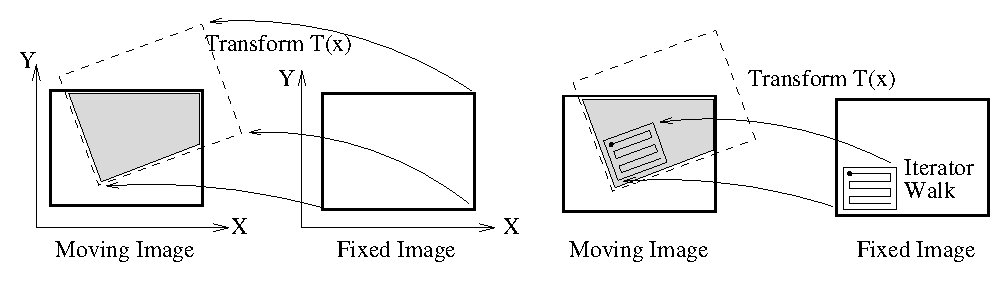
\includegraphics{ImageOverlap.eps}

An Image A is mapped over an image B by using a Transform


\subsection{Iterator Walking over a Region}

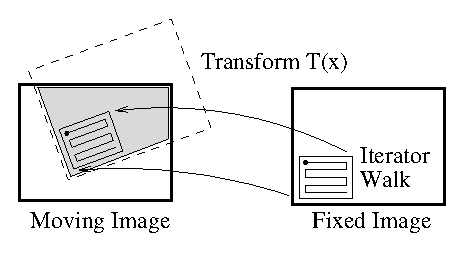
\includegraphics{ImageOverlapIterator.eps} 

An Iterator walking over a region of
B gets mapped on top of a blue region of A

\subsection{Need for an Interpolator}

The positions of the iterator are mapped
on non-grid positions in the image A 

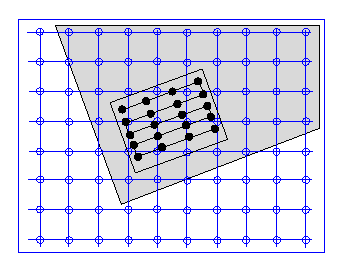
\includegraphics{ImageOverlapInterpolator.eps}

An interpolation is needed for estimating
the value of the image A at these non-grid positions.


\subsection{Overlaped regions }

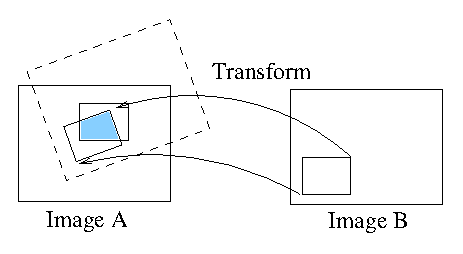
\includegraphics{ImageOverlapedRegions.eps}

Image metrics perform the computation over the intersection of a region in
image A and the map of a region in image B.



\fi

% the clearpage command helps to avoid orphans in the title of the next
% section.
\clearpage

\section{Metrics}
\label{sec:Metrics}
\ifitkFullVersion
%
%  This file is included by Registration.tex
%
%
%

\index{itk::Image\-To\-Image\-Metricv4}

In ITK, \doxygen{ImageToImageMetricv4} objects quantitatively measure how well
the transformed moving image fits the fixed image by comparing the gray-scale
intensity of the images. These metrics are very flexible and can work with any
transform or interpolation method and do not require reduction of the
gray-scale images to sparse extracted information such as edges.

The metric component is perhaps the most critical element of the registration
framework. The selection of which metric to use is highly dependent on the
registration problem to be solved. For example, some metrics have a large
capture range while others require initialization close to the optimal
position.  In addition, some metrics are only suitable for comparing images
obtained from the same imaging modality, while others can handle
inter-modality comparisons.
Unfortunately, there are no clear-cut rules as to how to choose a metric.

\index{itk::Image\-To\-Image\-Metricv4!GetValue()}
\index{itk::Image\-To\-Image\-Metricv4!GetDerivatives()}
\index{itk::Image\-To\-Image\-Metricv4!GetValueAndDerivatives()}

The matching Metric class controls most parts of the registration process
since it handles fixed, moving and virtual images as well as fixed and moving
transforms and interpolators.  The method \code{GetValue()} can be used to
evaluate the quantitative criterion at the transform parameters specified in
the argument.  Typically, the metric samples points within a defined region
of the virtual lattice.  For each point, the corresponding fixed and moving
image positions are computed using the fixed initial transform and the moving
transform with the specified parameters. Then, the fixed and moving interpolators
are used to compute the fixed and moving image's intensities at the mapped
positions. Details on this mapping are illustrated in Figures
\ref{fig:ImageOverlapIterator} and \ref{fig:ImageOverlapInterpolator} assuming
that virtual lattice is the same as the fixed image lattice, which is usually the
case in practice.

The metrics also support region-based evaluation. The \code{SetFixedImageMask()} and
\code{SetMovingImageMask()} methods may be used to restrict evaluation of the metric
within a specified region. The masks may be of any type derived from \doxygen{SpatialObject}.

Besides the measure value, gradient-based optimization schemes also require
derivatives of the measure with respect to each transform parameter. The
methods \code{GetDerivatives()} and \code{GetValueAndDerivatives()} can be
used to obtain the gradient information.


The following is the list of metrics currently available in ITKv4 registration framework:
\begin{itemize}
\item Mean squares\\ \doxygen{MeanSquaresImageToImageMetricv4}
\item Correlation \\ \doxygen{CorrelationImageToImageMetricv4}
\item Mutual information by Mattes \\ \doxygen{MattesMutualInformationImageToImageMetricv4}
\item Joint histogram mutual information \\ \doxygen{JointHistogramMutualInformationHistogramImageToImageMetricv4}
\item Demons metric \\ \doxygen{DemonsImageToImageMetricv4}
\item ANTS neighborhood correlation metric \\ \doxygen{ANTSNeighborhoodCorrelationImageToImageMetricv4}
\end{itemize}

Also, in case you are interested in using the legacy ITK registration framework,
the following is the list of metrics currently available in ITKv3:
\begin{itemize}
\item Mean squares\\ \doxygen{MeanSquaresImageToImageMetric}
\item Normalized correlation \\ \doxygen{NormalizedCorrelationImageToImageMetric}
\item Mean reciprocal squared difference \\ \doxygen{MeanReciprocalSquareDifferenceImageToImageMetric}
\item Mutual information by Viola and Wells \\ \doxygen{MutualInformationImageToImageMetric}
\item Mutual information by Mattes \\ \doxygen{MattesMutualInformationImageToImageMetric}
\item Kullback Liebler distance metric by Kullback and Liebler \\ \doxygen{KullbackLeiblerCompareHistogramImageToImageMetric}
\item Normalized mutual information \\ \doxygen{NormalizedMutualInformationHistogramImageToImageMetric}
\item Mean squares histogram \\ \doxygen{MeanSquaresHistogramImageToImageMetric}
\item Correlation coefficient histogram \\ \doxygen{CorrelationCoefficientHistogramImageToImageMetric}
\item Cardinality Match metric \\ \doxygen{MatchCardinalityImageToImageMetric}
\item Kappa Statistics metric\\ \doxygen{KappaStatisticImageToImageMetric}
\item Gradient Difference metric \\ \doxygen{GradientDifferenceImageToImageMetric}
\end{itemize}

In the following sections, we describe the ITKv4 metric types in detail.
You can check ITK descriptions in doxygen for details about ITKv3 metric classes.

For ease of notation, we will refer to the fixed image $f(\bf{X})$
and transformed moving image $(m \circ T(\bf{X}))$ as images $A$ and $B$.

\subsection{Mean Squares Metric}
\label{sec:MeanSquaresMetricv4}
\index{itk::Mean\-Squares\-Image\-To\-Image\-Metricv4}

The \doxygen{MeanSquaresImageToImageMetricv4} computes the mean squared
pixel-wise difference in intensity between image $A$ and $B$ over a user
defined region:

\begin{equation}
MS(A,B) = \frac{1}{N} \sum_{i=1}^N \left( A_i - B_i \right)^2
\end{equation}
\begin{center}
$A_i$ is the i-th pixel of Image A\\
$B_i$ is the i-th pixel of Image B\\
$N$ is the number of pixels considered
\end{center}

The optimal value of the metric is zero. Poor matches between images $A$ and
$B$ result in large values of the metric. This metric is simple to compute and
has a relatively large capture radius.

This metric relies on the assumption that intensity representing the same
homologous point must be the same in both images. Hence, its use is restricted
to images of the same modality. Additionally, any linear changes in the
intensity result in a poor match value.

\subsubsection{Exploring a Metric}
\label{sec:ExploringAMetric}

Getting familiar with the characteristics of the Metric as a cost function is
fundamental in order to find the best way of setting up an optimization process
that will use this metric for solving a registration problem. The following
example illustrates a typical mechanism for studying the characteristics of a
Metric. Although the example is using the Mean Squares metric, the same
methodology can be applied to any of the other metrics available in the
toolkit.

\ifitkFullVersion
\input{MeanSquaresImageMetric1.tex}
\fi


\subsection{Normalized Correlation Metric}
\label{sec:NormalizedCorrelationMetric}
\index{itk::Correlation\-Image\-To\-Image\-Metricv4}

The \doxygen{CorrelationImageToImageMetricv4} computes pixel-wise
cross-correlation and normalizes it by the square root of the autocorrelation
of the images:

\begin{equation}
NC(A,B) = -1 \times \frac{ \sum_{i=1}^N \left( A_i \cdot B_i \right) }
        { \sqrt { \sum_{i=1}^N A_i^2  \cdot \sum_{i=1}^N B_i^2 } }
\end{equation}
\begin{center}
$A_i$ is the i-th pixel of Image A\\
$B_i$ is the i-th pixel of Image B\\
$N$ is the number of pixels considered
\end{center}

Note the $-1$ factor in the metric computation. This factor is used to make the
metric be optimal when its minimum is reached.  The optimal value of the metric
is then minus one. Misalignment between the images results in small measure
values.  The use of this metric is limited to images obtained using the same
imaging modality.  The metric is insensitive to multiplicative factors between
the two images.  This metric produces a cost function with sharp peaks and
well-defined minima.  On the other hand, it has a relatively small capture radius.


\subsection{Mutual Information Metric}
\label{sec:MutualInformationMetric}

The \doxygen{MattesMutualInformationImageToImageMetricv4} computes the mutual
information between image $A$ and image $B$.  Mutual information (MI)
measures how much information one random variable (image intensity in one
image) tells about another random variable (image intensity in the other
image). The major advantage of using MI is that the actual form of the
dependency does not have to be specified.  Therefore, complex mapping between
two images can be modeled.  This flexibility makes MI well suited as a
criterion of multi-modality registration~\cite{Pluim2003}.

Mutual information is defined in terms of entropy. Let
\begin{equation}
H(A) = - \int p_A(a) \log p_A(a)\, da
\end{equation}
be the entropy of random variable $A$, $H(B)$ the entropy of
random variable $B$ and
\begin{equation}
H(A,B) = \int p_{AB}(a,b) \log p_{AB}(a,b)\,da\,db
\end{equation}
be the joint entropy of $A$ and $B$. If $A$ and $B$ are independent, then
\begin{equation}
p_{AB}(a,b) = p_A(a) p_B(b)
\end{equation}
and
\begin{equation}
H(A,B) = H(A) + H(B).
\end{equation}
However, if there is any dependency, then
\begin{equation}
H(A,B)<H(A)+H(B).
\end{equation}
The difference is called Mutual Information : \( I(A,B) \)
\begin{equation}
I(A,B)=H(A)+H(B)-H(A,B)
\end{equation}

\subsubsection{Parzen Windowing}


\begin{floatingfigure}[rlp]{0.5\textwidth}
 \centering
 \includegraphics[width=0.48\textwidth]{ParzenWindowing13.eps}
 \caption[Parzen Windowing in Mutual Information]{
In Parzen windowing, a continuous density function is constructed by
superimposing kernel functions (Gaussian function in this case) centered on the
intensity samples obtained from the image.\label{fig:ParzenWindowing}}
\end{floatingfigure}

In a typical registration problem, direct access to the marginal
and joint probability densities is not available and hence the
densities must be estimated from the image data. Parzen windows
(also known as kernel density estimators) can be used for this purpose.
In this scheme, the densities are constructed by taking intensity
samples $S$ from the image and super-positioning kernel functions
$K(\cdot)$ centered on the elements of $S$ as illustrated in
Figure \ref{fig:ParzenWindowing}:

A variety of functions can be used as the smoothing kernel with the
requirement that they are smooth, symmetric, have zero mean and
integrate to one. For example, boxcar, Gaussian and B-spline functions are
suitable candidates.  A smoothing parameter is used to scale the kernel
function.  The larger the smoothing parameter, the wider the kernel function
used and hence the smoother the density estimate. If the parameter is too
large, features such as modes in the density will get smoothed out.  On the
other hand, if the smoothing parameter is too small, the resulting density
may be too noisy. The estimation is given by the following equation.

\begin{equation}
p(a) \approx P^{*}(a) = \frac{1}{N} \sum_{s_j \in S} K\left(a - s_j\right)
\end{equation}

Choosing the optimal smoothing parameter is a difficult research problem and
beyond the scope of this software guide.  Typically, the optimal value of the
smoothing parameter will depend on the data and the number of samples used.

\subsubsection{Mattes et al. Implementation}
The implementation of mutual information metric available in ITKv4 follows
the method specified by Mattes et al. in \cite{Mattes2001} and is implemented
by the \doxygen{MattesMutualInformationImageToImageMetricv4} class.

\index{itk::Mattes\-Mutual\-Information\-Image\-To\-Image\-Metricv4}
In this implementation, only one set of intensity samples is drawn from the
image.  Using this set, the marginal and joint probability density function
(PDF) is evaluated at discrete positions or bins uniformly spread within the
dynamic range of the images. Entropy values are then computed by summing over
the bins.

\index{itk::Mattes\-Mutual\-Information\-Image\-To\-Image\-Metricv4!SetNumberOfHistogramBins()}

The number of spatial samples used is a ratio of the total number of samples
and is set using the \code{SetMetricSamplingPercentage()} method directly from
the registration framework \doxygen{ImageRegistrationMethodv4}. Also, The number
of bins used to compute the entropy values is set in the metric class
via the \code{SetNumberOfHistogramBins()} method.

Since the fixed image PDF does not contribute to the metric derivatives, it
does not need to be smooth. Hence, a zero-order (boxcar) B-spline kernel is
used for computing the PDF. On the other hand, to ensure smoothness, a
third-order B-spline kernel is used to compute the moving image intensity PDF. The
advantage of using a B-spline kernel over a Gaussian kernel is that the
B-spline kernel has a finite support region. This is computationally
attractive, as each intensity sample only affects a small number of bins and
hence does not require a $N \times N$ loop to compute the metric value.

During the PDF calculations, the image intensity values are linearly scaled
to have a minimum of zero and maximum of one. This rescaling means that a
fixed B-spline kernel bandwidth of one can be used to handle image data with
arbitrary magnitude and dynamic range.


\subsection{Normalized Mutual Information Metric}
Given two images, $A$ and $B$, the normalized mutual information may be computed as
\begin{equation}
NMI(A,B) = 1 + \frac{I(A,B)}{H(A,B)} = \frac{H(A) + H(B)}{H(A,B)}
\end{equation}
where the entropy of the images, $H(A)$, $H(B)$, the mutual
information, $I(A,B)$ and the joint entropy $H(A,B)$ are computed as mentioned
in \ref{sec:MutualInformationMetric}. Details of the implementation may be found in
\cite{Hajnal2001}.

\subsection{Demons metric}
\index{itk::Demons\-Image\-To\-Image\-Metricv4}

The implementation of the \doxygen{DemonsImageToImageMetricv4} metric is taken from
\doxygen{DemonsRegistrationFunction}.

The metric derivative can be calculated using image derivatives
either from the fixed or moving images. The default is to use fixed-image
gradients. See ObjectToObjectMetric::SetGradientSource to change
this behavior.

An intensity threshold is used, below which image pixels are considered
equal for the purpose of derivative calculation. The threshold can be
changed by calling \code{SetIntensityDifferenceThreshold}.

Note that this metric supports only moving transforms with local support and
with a number of local parameters that match the moving image dimension.
In particular, it's meant to be used with \doxygen{DisplacementFieldTransform}
and derived classes.


\subsection{ANTS neighborhood correlation metric}
\index{itk::ANTS\-Neighborhood\-Correlation\-Image\-To\-Image\-Metricv4}

The \doxygen{ANTSNeighborhoodCorrelationImageToImageMetricv4} metric computes
normalized cross correlation using a small neighborhood for each voxel between
two images, with speed optimizations for dense registration.

Around each voxel, the neighborhood is defined as a N-Dimensional
rectangle centered at the voxel. The size of the rectangle is 2*radius+1.
Normalized correlation between neighborhoods of the fixed image and the moving
image are averaged over the whole image as the final metric.
A radius less than 2 can be unstable. 2 is the default.

\fi

% the clearpage command helps to avoid orphans in the title of the next
% section.
\clearpage

\section{Optimizers}
\label{sec:Optimizers}
\ifitkFullVersion

\index{itk::ObjectToObjectOptimizer}
\index{itk::Single\-Valued\-NonLinear\-Vnl\-Optimizerv4}


\begin{figure}
\center
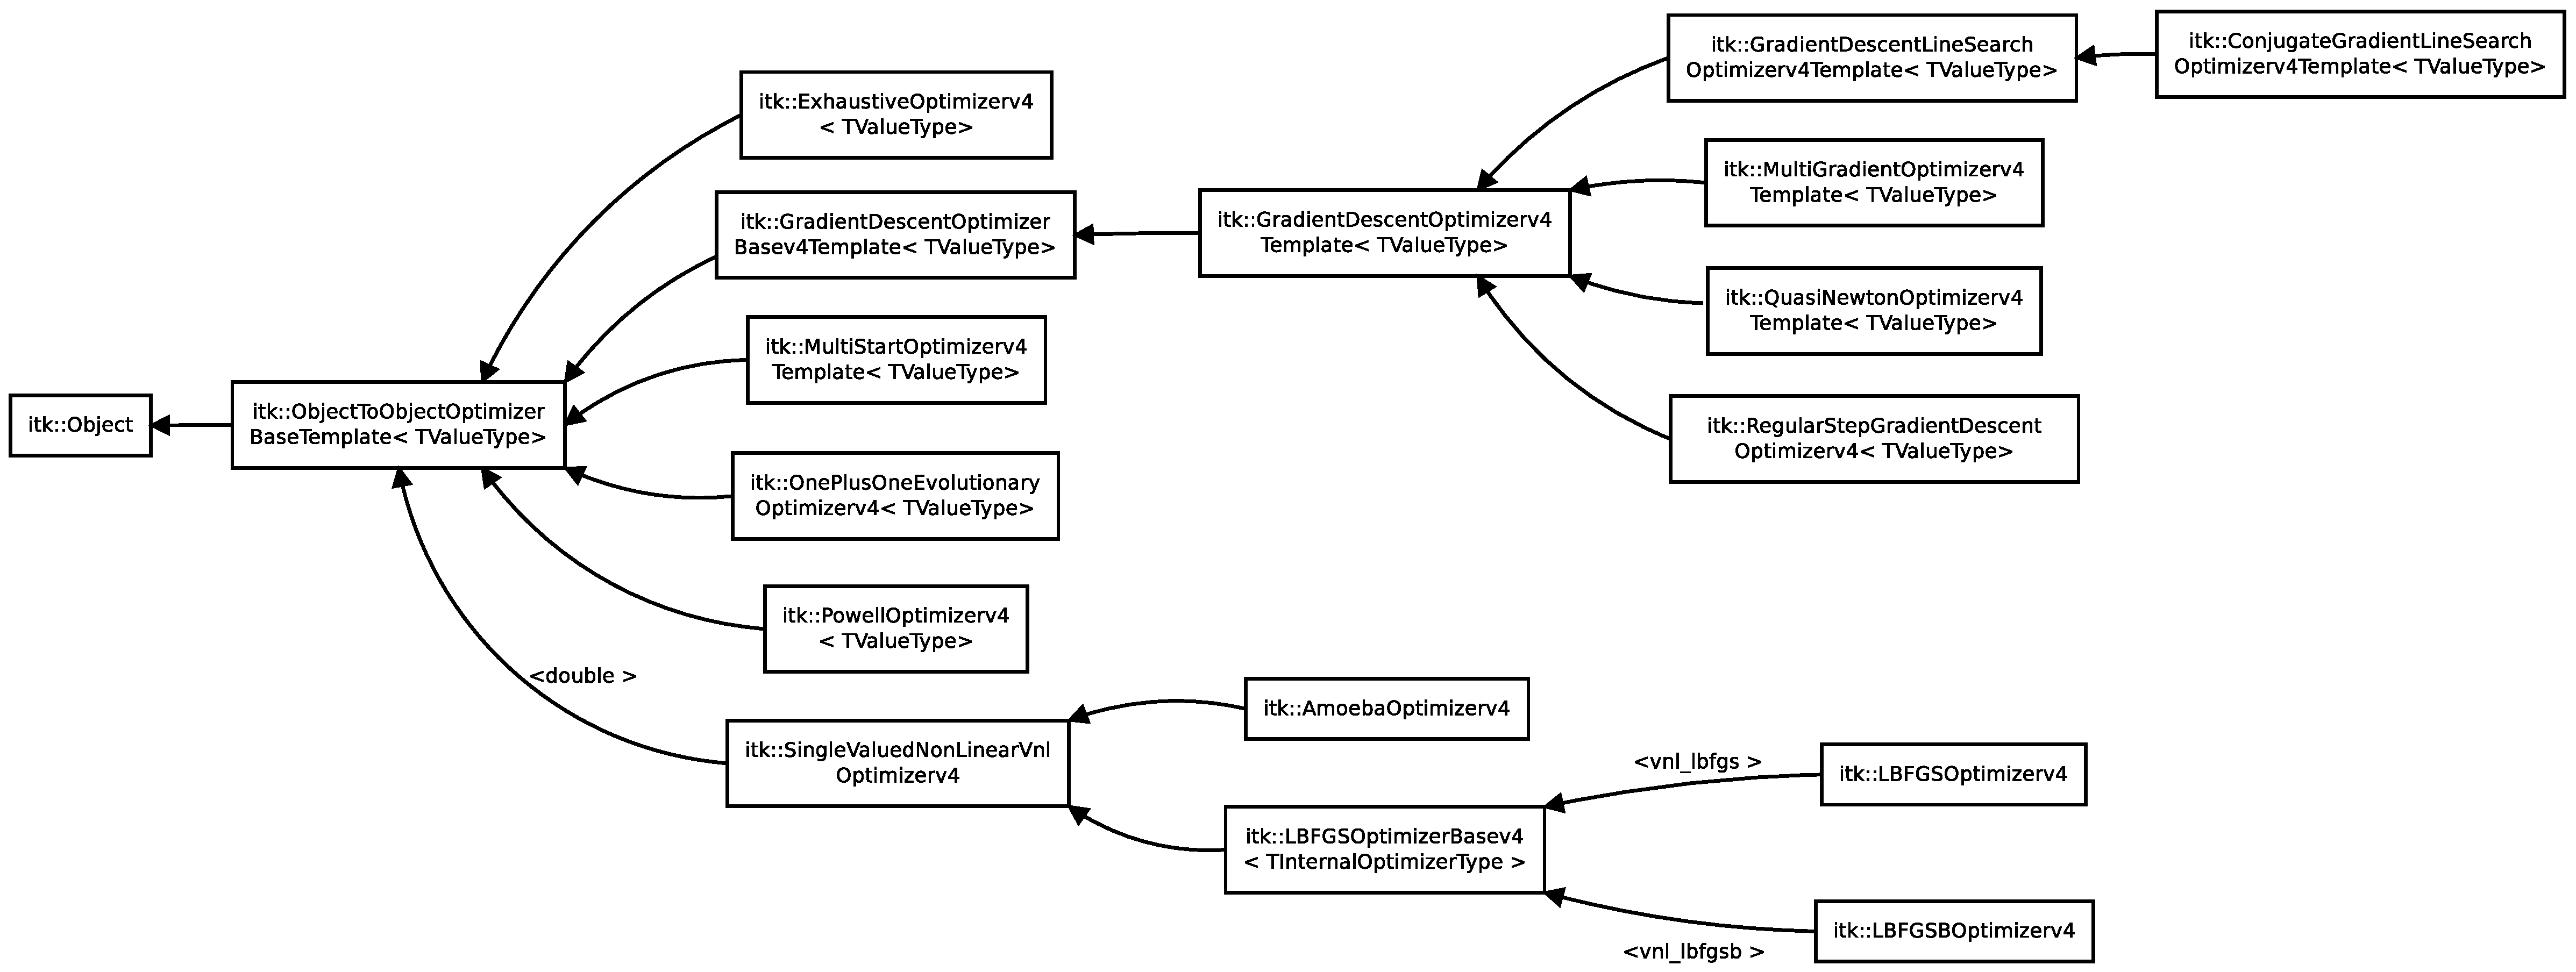
\includegraphics[width=\textheight,angle=90]{Optimizersv4Hierarchy.eps}
\itkcaption[Class diagram of the Optimizers hierarchy in ITKv4]{Class diagram of the
optimizersv4 hierarchy.}
\label{fig:Optimizersv4Hierarchy}
\end{figure}

Optimization algorithms are encapsulated as \doxygen{ObjectToObjectOptimizer}
objects within ITKv4. Optimizers are generic and can be used for applications
other than registration. Within the registration framework, subclasses of
\doxygen{SingleValuedNonLinearVnlOptimizerv4} are implemented as a wrap
around already implemented vnl classes.

\index{itk::ObjectToObjectOptimizer!SetMetric()}
\index{itk::ObjectToObjectOptimizer!StartOptimization()}
\index{itk::ObjectToObjectOptimizer!GetCurrentPosition()}

The basic input to an optimizer is a cost function or metric object. In the context
of registration, \doxygen{ImageToImageMetricv4} classes provide this functionality.
The metric is set using \code{SetInitialPosition()} and
the optimization algorithm is invoked by \code{StartOptimization()}.
Once the optimization has finished, the final parameters can be obtained
using \code{GetCurrentPosition()}.

\index{itk::ObjectToObjectOptimizer!SetScales()}
Some optimizers also allow rescaling of their individual parameters. This is
convenient for normalizing parameter spaces where some parameters have
different dynamic ranges. For example, the first parameter of
\doxygen{Euler2DTransform} represents an angle while the last two parameters
represent translations. A unit change in angle has a much greater impact on an
image than a unit change in translation. This difference in scale appears as
long narrow valleys in the search space making the optimization problem more
difficult. Rescaling the translation parameters can help to fix this problem.
Scales are represented as an \doxygen{Array} of doubles and set using
\code{SetScales()}.

\index{itk::ObjectToObjectOptimizer!SetScalesEstimator()}
Estimating the scales parameters can also be done automatically using the
\doxygen{OptimizerParameterScalesEstimatorTemplate} and its subclasses.
The scales estimator object is then set to the optimizer via
\code{SetScalesEstimator()}.

Despite the old version of ITK, there are only \emph{Single Valued} types
of optimizers available in ITKv4, which are suitable for dealing with cost
functions that return a single value. These are indeed the most common type
of cost functions, and are also known as \emph{Single Valued} functions.

The types of single valued optimizers currently available in ITKv4 are:

\index{itk::Gradient\-Descent\-Optimizerv4}
\index{itk::Regular\-Step\-Gradient\-Descent\-Optimizerv4}
\index{itk::Gradient\-Descent\-Line\-Search\-Optimizerv4}
\index{itk::Conjugate\-Gradient\-Line\-Search\-Optimizerv4}
\index{itk::Multi\-Gradient\-Optimizerv4}
\index{itk::Quasi\-Newton\-Optimizerv4}
\index{itk::Amoeba\-Optimizer}
\index{itk::LBFGS\-Optimizerv4}
\index{itk::LBFGSB\-Optimizerv4}
\index{itk::One\-Plus\-One\-Evolutionary\-Optimizerv4}
\index{itk::Powell\-Optimizerv4}
\index{itk::Exhaustive\-Optimizerv4}


\begin{itemize}

\item \textbf{Amoeba}: Nelder-Meade downhill simplex.  This optimizer is
actually implemented in the \code{vxl/vnl} numerics toolkit.  The ITK class
\doxygen{AmoebaOptimizerv4} is merely an adaptor class.

\item \textbf{Gradient Descent}: Advances parameters in the direction of the
gradient where the step size is governed by a learning rate
(\doxygen{GradientDescentOptimizerv4}).

\item \textbf{Gradient Descent Line Search}: Gradient descent with a golden
section line search. \doxygen{GradientDescentLineSearchOptimizerv4} implements
a simple gradient descent optimizer that is followed by a line search to find
the best value for the learning rate.

\item \textbf{Conjugate Gradient Descent Line Search}: Advances parameters in
the direction of the Polak-Ribiere conjugate gradient where a line search is
used to find the best value for the learning rate
(\doxygen{ConjugateGradientLineSearchOptimizerv4}).

\item \textbf{Quasi Newton}: Implements a Quasi-Newton optimizer with BFGS
Hessian estimation. Second order approximation of the cost function is usually
more efficient since it estimates the descent or ascent direction more precisely.
However, computation of Hessian is usually expensive or unavailable. Alternatively
Quasi-Newton methods can estimate a Hessian from the gradients in previous steps.
Here a specific Quasi-Newton method, BFGS, is used to compute the Quasi-Newton steps
(\doxygen{QuasiNewtonOptimizerv4}).

\item \textbf{LBFGS}: Limited memory Broyden, Fletcher, Goldfarb
and Shannon minimization. It is an adaptor to an optimizer in \code{vnl}
(\doxygen{LBFGSOptimizerv4}).

\item \textbf{LBFGSB}: A modified version of the LBFGS optimizer that allows to
specify bounds for the parameters in the search space.  It is an adaptor to an
optimizer in \code{netlib}. Details on this optimizer can be found
in~\cite{Byrd1995,Zhu1997} (\doxygen{LBFGSBOptimizerv4}).

\item \textbf{One Plus One Evolutionary}: Strategy that simulates the
biological evolution of a set of samples in the search space. This optimizer is
mainly used in the process of bias correction of MRI images
(\doxygen{OnePlusOneEvolutionaryOptimizerv4}). Details on this optimizer can be
found in~\cite{Styner2000}.

\item \textbf{Regular Step Gradient Descent}: Advances parameters in the
direction of the gradient where a bipartition scheme is used to compute
the step size (\doxygen{RegularStepGradientDescentOptimizerv4}).
This optimizer is also used for Versor transforms parameters, where the
current rotation is composed with the gradient rotation to produce the
new rotation versor. The translational part of the transform parameters
are updated as usually done in a vector space. It follows the definition
of versor gradients defined by Hamilton~\cite{Hamilton1866}

\item \textbf{Powell Optimizer}: Powell optimization method.  For an
N-dimensional parameter space, each iteration minimizes(maximizes) the function
in N (initially orthogonal) directions. This optimizer is described
in~\cite{Press1992}.  (\doxygen{PowellOptimizerv4}).

\item \textbf{Exhausive Optimizer}: Fully samples a grid on the parameteric space.
This optimizer is equivalent to an exahaustive search in a discrete grid defined
over the parametric space. The grid is centered on the initial position. The
subdivisions of the grid along each one of the dimensions of the parametric space
is defined by an array of number of steps
(\doxygen{ExhaustiveOptimizerv4}).

\end{itemize}

Figure \ref{fig:Optimizersv4Hierarchy} illustrates the full class hierarchy of
optimizers in ITK. Optimizers in the lower right corner are adaptor classes
to optimizers existing in the \code{vxl/vnl} numerics toolkit. The optimizers
interact with the \doxygen{CostFunction} class. In the registration framework
this cost function is reimplemented in the form of ImageToImageMetric.






\fi



\subsection{Registration using the One plus One Evolutionary Optimizer}
\label{sec:RegistrationOnePlusOne}
\ifitkFullVersion
\input{ImageRegistration11.tex}
\fi



\subsection{Registration using masks constructed with Spatial objects}
\label{sec:RegistrationSpatialObjects}
\ifitkFullVersion
\input{ImageRegistration12.tex}
\fi



\subsection{Rigid registrations incorporating prior knowledge}
\label{sec:RegistrationCentered2DTransform}
\ifitkFullVersion
\input{ImageRegistration13.tex}
\fi


% the clearpage command helps to avoid orphans in the title of the next
% section.
\clearpage

\section{Deformable Registration}
\label{sec:DeformableRegistration}
\ifitkFullVersion
%%%%%%%%%%%%%%%%%%%%%%%%%%%%%%%%%%%%%%%%%%%%%%%%%%%%%%%%%%%%%%%
%
%
%   This file is included in Registration.tex
%
%   Lablels and section entries are defined in that file.
%
%
%
%%%%%%%%%%%%%%%%%%%%%%%%%%%%%%%%%%%%%%%%%%%%%%%%%%%%%%%%%%%%%%%

 
\begin{figure} \center
\includegraphics[width=0.44\textwidth]{DeformableRegistration1CheckerboardBefore.eps}
\includegraphics[width=0.44\textwidth]{DeformableRegistration1CheckerboardAfter.eps}
\itkcaption[FEM-based deformable registration results]{Checkerboard comparisons
before and after FEM-based deformable registration.}
\label{fig:DeformableRegistration1Output}
\end{figure}

\ifitkFullVersion
\input{DeformableRegistration1.tex}
\fi

Figure \ref{fig:DeformableRegistration1Output} presents the results of
the FEM-based deformable registration applied to two time-separated
slices of a living mouse dataset.  Checkerboard comparisons of the two
images are shown before registration (left) and after registration
(right).  Both images were acquired from the same living mouse, the
first after inspiration of air into the lungs and the second after
exhalation.  Deformation occurs due to the elastic recoil of the lung
tissue and the relaxation of the diaphragm.

The following is a documented sample parameter file that can be used with this
deformable registration example.  This example demonstrates the setup of a
basic registration problem that does not use multi-resolution strategies.  As a
result, only one value for the parameters between \texttt{(\# of pixels per
element)} and \texttt{(maximum iterations)} is necessary.  In order to use a
multi-resolution strategy, you would have to specify values for those
parameters at each level of the pyramid.

\small
\verbatiminput{FiniteElementRegistrationParameters1.txt}
\normalsize



\fi

% the clearpage command helps to avoid orphans in the title of the next
% section.
\clearpage

\section{Demons Deformable Registration}
\label{sec:DemonsDeformableRegistration}
\ifitkFullVersion
%%%%%%%%%%%%%%%%%%%%%%%%%%%%%%%%%%%%%%%%%%%%%%%%%%%%%%%%%%%%%%%
%
%
%   This file is included in Registration.tex
%
%   Lablels and section entries are defined in that file.
%
%
%
%%%%%%%%%%%%%%%%%%%%%%%%%%%%%%%%%%%%%%%%%%%%%%%%%%%%%%%%%%%%%%%

% Brief description of the demons algorithm goes here

\input{DeformableRegistration2.tex} 


\fi

\section{Visualizing Deformation fields}
\label{sec:VisualizingDeformationFields}
\ifitkFullVersion
%%%%%%%%%%%%%%%%%%%%%%%%%%%%%%%%%%%%%%%%%%%%%%%%%%%%%%%%%%%%%%%
%
%
%   This file is included in Registration.tex
%
%   Lablels and section entries are defined in that file.
%
%
%
%%%%%%%%%%%%%%%%%%%%%%%%%%%%%%%%%%%%%%%%%%%%%%%%%%%%%%%%%%%%%%
Vector deformation fields may be visualized using ParaView.
ParaView \cite{ParaviewBook} is an open-source, multi-platform visualization application and uses the Visualization Toolkit as the data processing and rendering engine and has a user interface written using a unique blend of Tcl/Tk and C++. You may download it from http://paraview.org.

\subsection{Visualizing 2D deformation fields}
Let us visualize the deformation field obtained from Demons Registration algorithm generated from ITK/Examples/RegistrationITKv4/DeformableRegistration2.cxx.

Load the Deformation field in Paraview. (The deformation field must be capable of handling vector data, such as MetaImages). Paraview shows a color map of the magnitudes of the deformation fields as shown in \ref{fig:ParaviewScreenshot1}.

Covert the deformation field to 3D vector data using a {\it Calculator}. The Calculator may be found in the {\it Filter} pull down menu. A screenshot of the calculator tab is shown in Figure \ref{fig:ParaviewScreenshot2}. Although the deformation field is a 2D vector, we will generate a 3D vector with the third component set to 0 since Paraview generates glyphs only for 3D vectors. You may now apply a glyph of arrows to the resulting 3D vector field by using {\it Glyph} on the menu bar. The glyphs obtained will be very dense since a glyph is generated for each point in the data set. To better visualize the deformation field, you may adopt one of the following approaches.

Reduce the number of glyphs by reducing the number in {\it Max. Number of Glyphs} to reasonable amount. This uniformly downsamples the number of glyphs. Alternatively, you may apply a {\it Threshold} filter to the {\it Magnitude} of the vector dataset and then glyph the vector data that lies above the threshold. This eliminates the smaller deformation fields that clutter the display. You may now reduce the number of glyphs to a reasonable value.

Figure \ref{fig:ParaviewScreenshot3} shows the vector field visualized using Paraview by thresholding the vector magnitudes by 2.1 and restricting the number of glyphs to 100.

\begin{figure}
\center
\includegraphics[width=\textwidth]{ParaviewScreenshot1.eps}
\itkcaption[Deformation field magnitudes]{Deformation field magnitudes displayed using Paraview}
\label{fig:ParaviewScreenshot1}
\end{figure}

\begin{figure}
\center
\includegraphics[width=0.3\textwidth]{ParaviewScreenshot2.eps}
\itkcaption[Calculator]{Calculators and filters may be used to compute the vector magnitude, compose vectors etc.}
\label{fig:ParaviewScreenshot2}
\end{figure}

\begin{figure}
\center
\includegraphics[width=\textwidth]{ParaviewScreenshot3.eps}
\itkcaption[Visualized Def field]{Deformation field visualized using Paraview after thresholding and subsampling.}
\label{fig:ParaviewScreenshot3}
\end{figure}



\subsection{Visualizing 3D deformation fields}
Let us create a 3D deformation field. We will use Thin Plate Splines to warp a 3D dataset and create a deformation field. We will pick a set of point landmarks and translate them to provide a specification of correspondences at point landmarks. Note that the landmarks have been picked randomly for purposes of illustration and are not intended to portray a true deformation. The landmarks may be used to produce a deformation field in several ways. Most techniques minimize some regularizing functional representing the irregularity of the deformation field, which is usually some function of the spatial derivatives of the field. Here will we use {\it thin plate splines}. Thin plate splines minimize the regularizing functional

\begin{equation}
I[f(x,y)] = \iint (f^2_{xx} + 2 f^2_{xy} + f^2_{yy}) dx dy
\end{equation}
where the subscripts denote partial derivatives of f.

The code for this section can be found in ITK/Examples/RegistrationITKv4/ThinPlateSplineWarp.cxx

We may now proceed as before to visualize the deformation field using Paraview as shown in Figure \ref{fig:ParaviewScreenshot4}.

\begin{figure}
\center
\includegraphics[width=0.7\textwidth]{ParaviewScreenshot4.eps}
\itkcaption[Visualized Def field4]{3D Deformation field visualized using Paraview.}
\label{fig:ParaviewScreenshot4}
\end{figure}




\fi

\ifitkFullVersion
%%%%%%%%%%%%%%%%%%%%%%%%%%%%%%%%%%%%%%%%%%%%%%%%%%%%%%%%%%%%%%%
%
%
%   This file is included in DeformableRegistration.tex
%
%   Lablels and section entries are defined in that file.
%
%
%
%%%%%%%%%%%%%%%%%%%%%%%%%%%%%%%%%%%%%%%%%%%%%%%%%%%%%%%%%%%%%%
Let us register the deformed volumes generated by Thin plate warping in the
previous example using DeformableRegistration4.cxx. Since ITK is in general
N-dimensional, the only change in the example is to replace the
\code{ImageDimension} by 3.

The registration method uses B-splines and an LBFGS optimizer. The trace in
Table. \ref{tab:LBFGStrace} prints the trace of the optimizer through the
search space.

\begin{table}
\begin{center}
\begin{tabular}{\tableconfiguration}
\hline
\textbf{Iteration} &
\textbf{Function value} &
\textbf{$\|G\|$} &
\textbf{Step length} \\
\hline\hline
   1    &        156.981  &    14.911  & 0.202 \\
   2    &        68.956    &    11.774    &    1.500 \\
   3    &        38.146    &    4.802     &   1.500 \\
   4    &        26.690    &    2.515     &   1.500 \\
   5    &        23.295    &    1.106     &   1.500\\
   6    &        21.454    &    1.032     &   1.500\\
   7    &        20.322    &    1.557     &   1.500\\
   8    &        19.751    &    0.594     &   1.500\\
\hline
\end{tabular}
\end{center}
\itkcaption[LBFGS Optimizer trace]{LBFGS Optimizer trace.
\label{tab:LBFGStrace}}
\end{table}

Here $\|G\|$ is the norm of the gradient at the current estimate of the
minimum, $x$. ``Function Value" is the current value of the function, f(x).

The resulting deformation field that maps the moving to the fixed image is
shown in \ref{fig:DeformationFieldOutput}. A difference image of two slices
before and after registration is shown in
\ref{fig:DefRegistrationDiffScreenshot}. As can be seen from the figures, the
deformation field is in close agreement to the one generated from the Thin
plate spline warping.

\begin{figure}
\center
\includegraphics[width=0.6\textwidth]{ParaviewScreenshot5.eps}
\itkcaption[Deformation field output]{Resulting deformation field that maps the moving image to the fixed image.}
\label{fig:DeformationFieldOutput}
\end{figure}

\begin{figure}
\center
\includegraphics[width=0.44\textwidth]{DeformableRegistration4DiffBefore.eps}
\includegraphics[width=0.44\textwidth]{DeformableRegistration4DiffAfter.eps}
\itkcaption[Difference image]{Difference image from a slice before and after registration.}
\label{fig:DefRegistrationDiffScreenshot}
\end{figure}



\fi


% the clearpage command helps to avoid orphans in the title of the next
% section.
\clearpage



\section{Model Based Registration}
\label{sec:ModelBasedRegistration}
\ifitkFullVersion
%%%%%%%%%%%%%%%%%%%%%%%%%%%%%%%%%%%%%%%%%%%%%%%%%%%%%%%%%%%%%%%
%
%
%   This file is included in Registration.tex
%
%   Lablels and section entries are defined in that file.
%
%
%
%%%%%%%%%%%%%%%%%%%%%%%%%%%%%%%%%%%%%%%%%%%%%%%%%%%%%%%%%%%%%%%

\begin{floatingfigure}[rlp]{8cm}
  \centering
  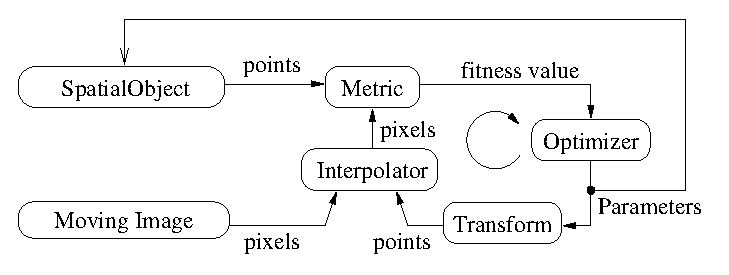
\includegraphics[width=7.5cm]{ModelToImageRegistrationComponentsDiagram.eps}
  \caption[Model to Image Registration Framework Components]{The basic
components of model based registration are an image, a spatial object, a
transform, a metric, an interpolator and an
optimizer.\label{fig:ModelToImageRegistrationComponentsDiagram}}
\end{floatingfigure}

This section introduces the concept of registering a geometrical model with
an image. We refer to this concept as \emph{model based registration} but
this may not be the most widespread terminology. In this approach, a
geometrical model is built first and a number of parameters are identified in
the model. Variations of these parameters make it possible to adapt the model
to the morphology of a particular patient. The task of registration
is then to find the optimal combination of model parameters that will
make this model a good representation of the anatomical structures
contained in an image.

For example, let's say that in the axial view of a brain image we can roughly
approximate the skull with an ellipse. The ellipse becomes our simplified
geometrical model, and registration is the task of finding the best center for
the ellipse, the measures of its axis lengths and its orientation in the plane.
This is illustrated in Figure~\ref{fig:ModelToImageRegistrationConcept}.  If we
compare this approach with the image-to-image registration problem, we can see
that the main difference here is that in addition to mapping the spatial
position of the model, we can also customize internal parameters that change
its shape.

Figure~\ref{fig:ModelToImageRegistrationComponentsDiagram}   illustrates  the
major  components of  the registration  framework in  ITK when  a  model-based
registration problem is configured. The basic input data for the registration
is  provided by  pixel data  in an  \doxygen{Image} and  by  geometrical data
stored in a  \doxygen{SpatialObject}. A metric has to be  defined in order to
evaluate the fitness between the model  and the image. This fitness value can
be  improved by  introducing variations  in  the spatial  positioning of  the
SpatialObject and/or  by changing its  internal parameters. The  search space
for the optimizer  is now the composition of the  transform parameter and the
shape internal parameters.

This same approach can be considered a segmentation technique, since once the
model has been optimally superimposed on the image we could label pixels
according to their associations with specific parts of the model. The
applications of model to image registration/segmentation are endless.
The main advantage of this approach is probably that, as opposed to image-to-image
registration, it actually provides \emph{Insight} into the anatomical structure
contained in the image. The adapted model becomes a condensed representation of
the essential elements of the anatomical structure.

\begin{figure}
\center
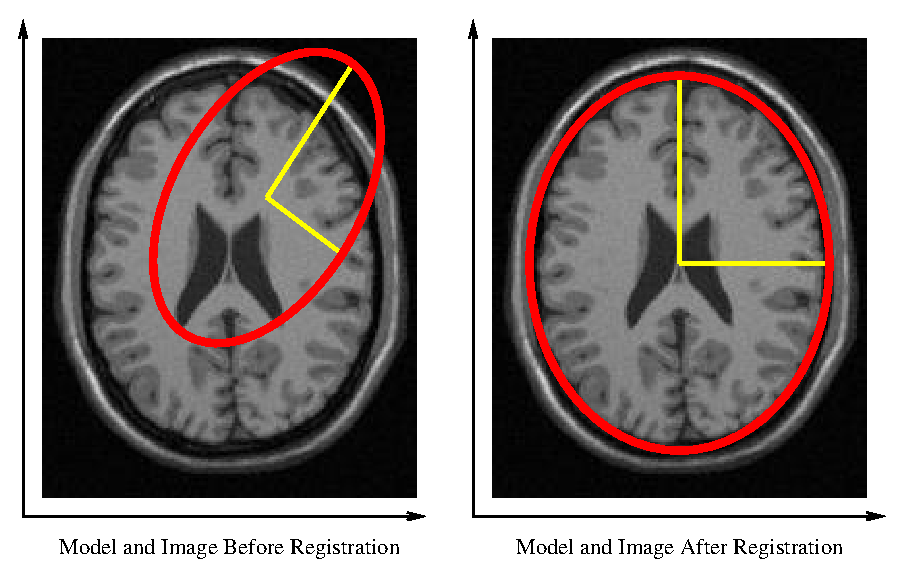
\includegraphics[width=0.8\textwidth]{ModelToImageRegistrationConcept.eps}
\itkcaption[Model to Image Registration Framework Concept]{Basic concept of
  Model-to-Image registration.  A simplified geometrical model (ellipse) is
    registered against an anatomical structure (skull)  by applying a spatial
    transform and modifying the model internal parameters. This image is not
    the result of an actual registration, it is shown here only with the
    purpose of illustrating the concept of model to image registration.}
\label{fig:ModelToImageRegistrationConcept}
\end{figure}


ITK provides a hierarchy of classes intended to support the construction of
shape models. This hierarchy has the SpatialObject as its base class.
A number of basic functionalities are defined at this level, including the
capacity to evaluate whether a given point is \emph{inside} or \emph{outside} of the
model, form complex shapes by creating hierarchical
conglomerates of basic shapes, and support basic spatial
parameterizations like scale, orientation and position.

The following sections present examples of the typical uses of these powerful
elements of the toolkit.

\ifitkFullVersion
\input{ModelToImageRegistration1.tex}
\fi





\fi


\section{Point Set Registration}
\label{sec:PointSetRegistration}

PointSet-to-PointSet registration is a common problem in medical image
analysis. It usually arises in cases where landmarks are extracted from images
and are used for establishing the spatial correspondence between the images.
This type of registration can be considered to be the simplest case of
feature-based registration. In general terms, feature-based registration is
more efficient than the intensity based method that we have presented so far.
However, feature-base registration brings the new problem of identifying and
extracting the features from the images, which is not a minor challenge.

The two most common scenarios in PointSet to PointSet registration are

\begin{itemize}
\item Two PointSets with the same number of points, and where each point in one
set has a known correspondence to exactly one point in the second set.
\item Two PointSets without known correspondences between the points of one set
and the points of the other. In this case the PointSets may have different
numbers of points.
\end{itemize}

The first case can be solved with a closed form solution when we are dealing
with a Rigid or an Affine Transform~\cite{Horn1987}. This is done in ITK with
the class \doxygen{LandmarkBasedTransformInitializer}. If we are interested in
a deformable Transformation then the problem can be solved with the
\doxygen{KernelTransform} family of classes, which includes Thin Plate Splines
among others~\cite{Rohr2001}. In both circumstances, the availability o f
correspondences between the points make possible to apply a straight forward
solution to the problem.


The classical algorithm for performing PointSet to PointSet registration is the
Iterative Closest Point (ICP) algorithm.  The following examples illustrate how
this can be used in ITK.



\subsection{Point Set Registration in 2D}
\label{sec:PointSetRegistrationIn2D}

\ifitkFullVersion
\input{IterativeClosestPoint1.tex}
\fi




\subsection{Point Set Registration in 3D}
\label{sec:PointSetRegistrationIn3D}

\ifitkFullVersion
\input{IterativeClosestPoint2.tex}
\fi



\subsection{Point Set to Distance Map Metric}
\label{sec:PointSetToDistanceMapMetric}

\ifitkFullVersion
\input{IterativeClosestPoint3.tex}
\fi



\section{Registration Troubleshooting}
So you read the previous sections, you wrote the code, it compiles and links fine,
but when you run it the registration results are not what you were expecting.
In that case, this section is for you. This is a compilation of the most common
problems that users face when performing image registration. It provides explanations
on the potential sources of the problems, and advice on how to deal with those problems.

Most of the material in this section has been taken from frequently asked questions of
the ITK users list.


\subsection{Too many samples outside moving image buffer}


http://public.kitware.com/pipermail/insight-users/2007-March/021442.html

This is a common error message in image registration.

It means that at the current iteration of the optimization,
the two images as so off-registration that their spatial
overlap is not large enough for bringing them back into
registration.

The common causes of this problem are:

\begin{itemize}
\item Poor initialization:    You must initialize the transform properly.
Please read the ITK Software Guide http://www.itk.org/ItkSoftwareGuide.pdf  for
a description of the use of the CenteredTransformInitializer class.
\item Optimzer steps too large. If you optimizer takes steps that are too
large, it risks to become unstable and to send the images too far appart.  You
may want to start the optimizer with a maximum step lenght of 1.0, and only
increase it once you have managed to fine tune all other registration
parameters.

Increasing the step length makes your program faster, but it also makes it more
unstable.



\item Poor set up o the transform parameters scaling.  This is extremely
critical in registration. You must make sure that you balance the relative
difference of scale between the rotation parameters and the translation
parameters.

In typical medical datasets such as CT and MR, translations are measured in
millimeters, and therefore are in the range of -100:100, while rotations are
measured in radians, and therefore they tend to be in the range of   -1:1.


A rotation of 3 radians is catastrophic, while a translation of 3 millimeters
is rather inoffensive.  That difference in scale is the one that must be
accounted for.
\end{itemize}



\subsection{General heuristics for parameter fine-tunning}





http://public.kitware.com/pipermail/insight-users/2007-March/021435.html

Here is some advice on how to fine tune the parameters
of the registration process.


1) Set Maximum step length to 0.1 and do not change it
   until all other parameters are stable.

2) Set Minimum step length to 0.001 and do not change it.

   You could interpret these two parameters as if their
   units were radians. So, 0.1 radian = 5.7 degrees.


3) Number of histogram bins:

    First plot the histogram of your image using the
    example program in

    Insight/Examples/Statistics/ImageHistogram2.cxx

    In that program use first a large number  of bins
    (for example 2000) and identify the different
    populations of intensity level and to what anatomical
    structures they correspond.

    Once you identify the anatomical structures in the
    histogram, then rerun that same program with less
    and less number of bins, until you reach the minimun
    number of bins for which all the tissues that are important
    for your application, are still distinctly differentiated in the
    histogram.  At that point, take that number of bins and
    us it for your Mutual Information metric.


4)  Number of Samples:
    The trade-off with the number of samples is the following:

    a) computation time of registration is linearly proportional
       to the number of samples
                                                                                                                        b) the samples must be enough to significantly populate
                                                                                                                           the joint histogram.
                                                                                                                        c) Once the histogram is populated, there is not much
                                                                                                                           use in adding more samples.
Therefore do the following:

Plot the joint histogram of both images, using the number
of bins that you selected in item (3). You can do this by
modifying the code of the example:

Insight/Examples/Statistics/
ImageMutualInformation1.cxx
you have to change the code to print out the values
of the bins. Then use a plotting program such as gnuplot,
or Matlab, or even Excel and look at the distribution.
The number of samples to take must be enough
for producing the same "appearance" of the joint histogram.
As an arbitrary rule of thumb you may want to start using
a high number of samples (80% ~ 100%). And do not
change it until you have mastered the other parameters
of the registration.  Once you get your registration to converge
you can revisit the number of samples and reduce it in order
to make the registration run faster. You can simply reduce it
until you find that the registration becomes unstable. That's
your critical bound for the minimum number of samples.
Take that number and multiply it by the magic number 1.5,
to send it back to a stable region, or if your application is
really critical, then use an even higher magic number x2.0.

This is just engineering: you figure out what is the minimal
size of a piece of steel that will support a bridge, and then
you enlarge it to keep it away from the critical value.

5)  The MOST critical values of the registration process are the
scaling parameters that define the proportions between
the parameters of the transform. In your case, for an Affine
Transform in 2D, you have 6 parameters. The first four are
the ones of the Matrix, and the last two are the translation.
The rotation matrix value must be in the ranges of radians
which is typically [ -1 to 1 ], while the translation values are
in the ranges of millimeters (your image size units).
You want to start by setting the scaling of the matrix
parameters to 1.0, and the scaling of the Translation
parameters to the holy esoteric values:

1.0   /  (  10.0 * pixelspacing[0]  *  imagesize[0]  )
1.0   /  (  10.0 * pixelspacing[1]  *  imagesize[1]  )

This is telling the optimizer that you consider that rotating
the image by 57 degrees is as "significant" as translating
the image by half its physical extent.

Note that esoteric value has included the arbitrary number
10.0 in the denominator, for no other reason that we have
been lucky when using that factor. This of course is just a
supersticion, so you should feel free to experiment with
different values of this number.

Just keep in mind that what the optimizer will do is to
"jump" in a paramteric space of 6 dimension, and that the
component of the jump on every dimension will be proporitional
to 1/scaling factor * OptimizerStepLenght.     Since you put
the optimizer Step Length to 0.1, then the optimizer will start
by exploring the rotations at jumps of about 5degrees, which
is a conservative rotation for most medical applications.

If you have reasons to think that your rotations are larger or
smaller, then you should modify the scaling factor of the  matrix
parameters accordingly.

In the same way, if you thinkl that 1/10 of the image size is too
large as the first step for exploring the translations, then you
should modify the scaling of  translation parameters accordingly.



In order to drive all these you need to analyze the feedback that
the observer is providing you. For example, plot the metric values,
and plot the translation coordinates so that you can get a feeling
of how the registration is behaving.


Note also that image registration is not a science. it is a pure
engineerig practice, and therefore, there are no correct answers,
nor "truths" to be found. It is all about how much quality your want,
and how must computation time, and development time are you
willing to pay for that quality. The "satisfying" answer for your
specific application must be found by exploring the trade-offs
between the different parameters that regulate the image
registration process.

If you are proficient in VTK you may want to consider attaching
some visualization to the Event observer, so that you can have
a visual feedback on the progress of the registration. This is a
lot more productive than trying to interpret the values printed
out on the console by the observer.

\input{DF04-Segmentation.tex}
\input{DF05-Statistics.tex}

\backmatter

%%%%%%%%%%%%%%%%%%%%%%%%%%%%%%%%%%%%%%%%%
%
%  Insert the bibliography using BibTeX
%
%%%%%%%%%%%%%%%%%%%%%%%%%%%%%%%%%%%%%%%%%

\bibliographystyle{plain}
\bibliography{\bibtexdatabasepath}


%%%%%%%%%%%%%%%%%%%%%%%%%%%%%%%%%%%%%%%%%
%
%  Insert the Index file
%
%%%%%%%%%%%%%%%%%%%%%%%%%%%%%%%%%%%%%%%%%

\InputIfFileExists{001-ITKSoftwareGuide-Book2.ind}


%\ifitkPrintedVersion
%\cleardoublepage
%\input{DG05-MarketingMaterial.tex}
%\fi

\end{document}
